\documentclass[12pt,a4paper]{article}

\usepackage{hyperref}
\usepackage{graphicx}
\usepackage{caption}
\usepackage{subcaption}
\usepackage{amssymb}
\usepackage{amsmath}
\usepackage{amsthm}
\usepackage[margin=19mm]{geometry}
\usepackage{natbib}
\usepackage{bm}
\usepackage[toc,page]{appendix}
\usepackage{booktabs}
%\usepackage{url}
%\usepackage{fancyhdr}
%\usepackage{fancyvrb}
\usepackage{lscape}
%\usepackage{pdfsync}
\usepackage{rotating}
\usepackage{multirow}
\usepackage[nodisplayskipstretch]{setspace} \setstretch{1.5}
\let\oldv\verbatim
\def\verbatim{\par\setstretch{0.9}\oldv}
\usepackage[table]{xcolor}
\usepackage{algorithm,algorithmic}
%\usepackage{fancyhdr}

%\setlength{\headheight}{10pt}
%\pagestyle{fancyplain}
%\fancyhf{}
%\fancyfoot[R]{\thepage}
%\fancyhead[R]{\nouppercase{\leftmark}}
%\fancypagestyle{plain}{%
%\fancyhead{} % get rid of headers
%\renewcommand{\headrulewidth}{0pt} % and the line
%}

%\renewcommand{\headrulewidth}{0.5pt} %Do not print a rule below the header
%\renewcommand{\footrulewidth}{0pt} %Do not print a rule above the footer

\bibpunct{(}{)}{;}{a}{,}{,}

%\renewenvironment{tabbing}{\linebreak \texttt \sl}{\linebreak}

\newcommand{\undertilde}[1]{\underset{\widetilde{}}{#1}}
\newcommand{\threeScript}[3]{
	\!\begin{smarray}{l}
  		{#1}\\ \hlx{s[-5pt]}
  		{#2}\\ \hlx{s[-5pt]}
  		{#3}
 	 \end{smarray}
}
\renewcommand{\baselinestretch}{1.5}
\setlength{\abovecaptionskip}{3pt}
\setlength{\belowcaptionskip}{3pt}

\newtheorem{mydef}{Definition}

\floatname{algorithm}{Pseudocode}

\hypersetup{
    bookmarks=true,         % show bookmarks bar?
    unicode=false,          % non-Latin characters in Acrobat’s bookmarks
    pdftoolbar=true,        % show Acrobat’s toolbar?
    pdfmenubar=true,        % show Acrobat’s menu?
    pdffitwindow=false,     % window fit to page when opened
    pdfstartview={FitH},    % fits the width of the page to the window
    pdftitle={My title},    % title
    pdfauthor={Author},     % author
    pdfsubject={Subject},   % subject of the document
    pdfcreator={Creator},   % creator of the document
    pdfproducer={Producer}, % producer of the document
    pdfkeywords={keyword1} {key2} {key3}, % list of keywords
    pdfnewwindow=true,      % links in new window
    linktoc = page,
    colorlinks=true,       % false: boxed links; true: colored links
    linkcolor=blue,          % color of internal links
    citecolor=blue,        % color of links to bibliography
    filecolor=magenta,      % color of file links
    urlcolor=cyan           % color of external links
}


%###################################################################################################
%Writing starts here!!
%
%###################################################################################################

\begin{document}
\title{Estimating the variance component and effective degrees of freedom}
\author{Kevin Chang}
\date{\today}
\maketitle
%\tableofcontents

\section{Introduction}
\label{sec:intro}
This thesis has presented a method in constructing the theoretical ANOVA table for the two-phase experiments (in Chapter 2). In Chapter 3 and 4, the search methods for optimal two-phase design has developed. The designs of the Phase 1 experiments were considered are completely randomised design (CRD), randomised block design (RBD) and balanced incomplete block design (BIBD). The theoretical ANOVA tables has shown to be a very useful tool for comparing the properties of between the optimal two-phase designs. Therefore, so far, this thesis has presented two tools: a way to study the two-phase designs and a method in designing an optimal two-phase designs. This section give a third tool in recovering the information from the Between Runs stratum.

\cite{Jarrett2008} demonstrated that despite having the same number of biological and technical replicates, the outcome of an micro-array experiment can be affected by the type of design used. MudPIT-iTRAQ experiments have their own set of unique problems. When using iTRAQ experiment, either the 4-plex or 8-plex system can be used which allows the researchers to measure 4 or 8 samples simultaneously. Consider the example where the Phase 1 experiment is arranged in CRD with $v = 2$ treatments and $r_b = 3$ biological replicates, the total number of animals is 6. If the 4-plex system is used, the animals cannot be to allocated to runs in such way that the animal is orthogonal to runs. Hence, some animal information can be in the Between Runs stratum. This chapter aims to illustrated on how to recover some of this animal information from the Between Runs stratum which effectively has higher degrees of freedom (DF) for conducting the test for the treatment effects. This newly adjusted DF is also known as \emph{effective degrees of freedom} (EDF). 

The EDF are computed based on the variance components (VC) estimated. Two methods in estimating the VC are discused in this chapter. The first method uses the linear combination (LC) of the expected mean squares (EMS) utilising the theoretical ANOVA table. The second method attempts to improve the estimation of the VC estimates by using the restricted maximum likelihood (REML) technique \citep{Patterson1971}. The EDF are then computed from the first two moments of an approximate chi-square distribution and based on the Satterthwaite approximation \citep{Jarrett2008, Satterthwaite1946}.
 
This chapter first uses an optimal design to illustrate the estimation of VC using LC or REML methods. Based on the VC estimates, the computation of EDF is then shown. The EDF of the different two-phase designs are then compared using the an identical Phase 1 experiment. 

\section{An illustrative example}
\label{sec:expDes}
The simplest example of a two-phase experiment where the first phase is arranged in CRD is presented in this section. The Phase 1 experiment consists of 2 treatments, 3 biological replicates and 2 technical replicates. This means there are total of 12 observations that can be measured in the Phase 2 experiment. Providing that 4-plex system is used in the Phase 2 experiment, 3 runs are required to measure all 12 samples generated from the Phase 1 experiment. An example of optimal two-phase design is presented in Table~\ref{tab:aniDes1} and \ref{tab:trtDes1}.

\begin{table}[ht]
\centering
\caption{Animal allocation to runs and tags.}
\begin{tabular}{c|cccc}
 & \multicolumn{4}{c}{{\bf Tag}} \\
{\bf Run}  & 114 & 115 & 116 & 117 \\ 
\hline 
1 & D & C & F & E \\  
2 & C & D & E & F \\  
3 & B & B & A & A \\ 
\end{tabular} 
\label{tab:aniDes1}
\end{table}

\begin{table}[ht]
\centering
\caption{Treatment allocation to runs and tags.}
\begin{tabular}{c|cccc}
 & \multicolumn{4}{c}{{\bf Tag}} \\
{\bf Run}  & 114 & 115 & 116 & 117 \\ 
\hline 
1 & b & a & b & a \\  
2 & a & b & a & b \\  
3 & b & b & a & a \\  
\end{tabular} 
\label{tab:trtDes1}
\end{table}

The theoretical ANOVA table generated from this optimal design can be expressed in Table~\ref{tab:Phase2ANOVA}. Notice this theoretical ANOVA table contains an extra column with the mean squares (MS) which are computed from the experimental data. Since the VC are estimated from the MS that are free of the fixed effects, there are four MS of interest in this theoretical ANOVA table denoted by $s_i^2, \; (i = 1,\dots, 4).$ The EMS of the corresponding MS, $s_i^2$, can be denoted by $\xi_i^2$. Hence, the vectors of MS and EMS, denoted by $\bm{s^2}$ and $\bm{\xi^2}$, respectively, are used to illustrate on the estimation the VC and EDF in the following section.

\begin{table}[ht]
\centering
\caption{Theoretical ANOVA table of the two-phase experiment}
\begin{tabular}{lrllll} 
\toprule 
\multicolumn{1}{l}{\textbf{Source of Variation}} & \multicolumn{1}{l}{\textbf{DF}}& \multicolumn{1}{l}{\textbf{MS}} & \multicolumn{1}{l}{\textbf{EMS}}& \multicolumn{1}{l}{$\bm{E_{\gamma}}$}&\multicolumn{1}{l}{$\bm{E_{\tau}}$}\\ 
\midrule 
Between Runs & & &  & & \\ 
\quad Between Animals & $1$ &$s_1^2$ & $ \sigma^2+2\sigma_{A}^2+4\sigma_{R}^2$ & & \\ 
\quad Within Animals & $1$ &$s_2^2$& $\sigma^2+4\sigma_{R}^2$ & & \\ \hline 
Within Runs &  &&  & & \\ 
\quad Between Animals &&  &  & & \\ 
\quad \quad Tag & $1$ && $\sigma^2+2\sigma_{A}^2+3\theta_{\gamma}+\frac{2}{3}\theta_{\tau}$ &$1$ & $\frac{1}{9}$\\ 
\quad \quad Treatment & $1$ & & $\sigma^2+2\sigma_{A}^2+\frac{16}{3}\theta_{\tau}$ & & $\frac{8}{9}$\\ 
\quad \quad Residual & $2$ &$s_3^2$& $\sigma^2+2\sigma_{A}^2$ & & \\ \hline 
\quad Within Animals &  &&  & & \\ 
\quad \quad Tag & $2$ && $\sigma^2+3\theta_{\gamma}$ &$1$ & \\ 
\quad \quad Residual & $3$ &$s_4^2$& $\sigma^2$ & & \\ 
\bottomrule 
\end{tabular} 
\label{tab:Phase2ANOVA} 
\end{table} 

\section{Estimation of the variance components}
\label{sec:estVC}
This section illustrates the estimation of the VC using LC and REML methods based on the example presented in Section~\ref{sec:expDes}. Thus, the VC to be estimated are the VC of measurement error, between animals and between runs which are denoted by $\sigma^2$, $\sigma_A^2$ and $\sigma_R^2$, respectively. However, the methods presented can readily be used on the different two-phase experiments with different set of design parameters. 

\subsection{Estimation of VC using the LC method} 
The LC method requires the coefficient of VC in the EMS from the theoretical ANOVA table as shown in Table~\ref{tab:Phase2ANOVA}. The $\sigma^2$ can be obtained directly from the MS of the residual in the Within Animals Within Runs stratum, i.e.\ $s_4^2$. The $\sigma_A^2$ is calculated from $\dfrac{s_3^2 - s_4^2}{2}.$ The $\sigma_R^2$ is calculated from $\dfrac{s_2^2 - s_4^2}{4}.$ 
  
\subsection{Estimation of VC using the REML method}  
The second method is attempting to use a REML technique to estimate the VC. This REML technique is known as the Fisher's scoring algorithm which is an iterative procedure which can be used to solve maximum likelihood equations. The algorithm stops when the difference between the VC from two consecutive iterations is less than 1e-7. 

The formula for Fisher's scoring algorithm can be written as 
\begin{equation}\label{eq:fisherScore}
\bm{\sigma}_{t+1}= \bm{\sigma}_t+\mathcal{I}^{-1}(\bm{\sigma}_t )S(\bm{\sigma}_t )
\end{equation}
where $\bm{\sigma}_{t}$ and $\bm{\sigma}_{t+1}$ are vectors of VC estimates at the $t$th and $(t+1)$th iterations, respectively. For current example, the $\bm{\sigma}$ consists of $\sigma^2$, $\sigma_A^2$ and $\sigma_R^2$. The inverse of the Fisher information matrix and score function with the function of $\bm{\sigma}_t$ are denoted by $\mathcal{I}^{-1}(\bm{\sigma}_t )$ and $S(\bm{\sigma}_t )$, respectively. Thus, in order to estimate the VC using the Fisher scoring algorithm, the score function and Fisher information matrix are needed to be defined and will be shown in the remaining of this section. 

\subsection{Constructing the score function and Fisher information matrix} 
The mean squares $s_i^2$ are assumed to have a chi-square distribution, i.e.\
\begin{equation}
s_i^2 \sim \dfrac{\xi_i^2}{\upsilon_i} \chi_{\upsilon_i}^2, \;  (i = 1,\dots,4), 
\end{equation}
where $\upsilon_i$ denotes the DF corresponding to $s_i^2$. The log-likelihood of $s_i^2$ can be shown as 
\[L(\xi_i^2;s_i^2) = constant - \sum_{i = 1}^{4}\left[ \dfrac{\upsilon_i log(\xi_i^2)}{2} + \dfrac{\upsilon_i s_i^2}{2\xi_i^2}\right], \;  (i = 1,\dots,4). \]   
The score is the first derivative of the log-likelihood function with respect to the $i$th element of EMS, $\xi_i^2$, i.e.\
\[\dfrac{\partial L(\xi_i^2;s_i^2)}{\partial \xi_i^2} = \dfrac{\upsilon_i (s_i^2 - \xi_i^2)}{2\xi_i^4}, \;  (i = 1,\dots,4).\]
Since $\bm{\xi^2}$ is a vector of four elements for the current example, the score function can be re-written as a vector shown as 
\[S(\bm{\xi^2}) = \dfrac{\partial L(\bm{\xi^2};\bm{s^2})}{\partial \bm{\xi^2}} = 
\begin{pmatrix}               
\dfrac{\upsilon_1 (s_1^2 - \xi_1^2)}{2\xi_1^4} \\
 \dfrac{\upsilon_2 (s_2^2 - \xi_2^2)}{2\xi_2^4} \\
 \dfrac{\upsilon_3 (s_3^2 - \xi_3^2)}{2\xi_3^4}  \\
\dfrac{\upsilon_4 (s_4^2 - \xi_4^2)}{2\xi_4^4}  \\
\end{pmatrix}. \]

The Fisher information is defined as the variance of the score. As shown above, the first derivative of the log-likelihood function with respected to $\xi_i^2$ is the score. The negative expectation of the second derivative of the log-likelihood function with respected to $\xi_i^2$ is therefore the Fisher information. This is also know as the expected Fisher Information.

Since $\bm{\xi^2}$ is a vector of four elements, the negative expectation of the second partial derivative of the log-likelihood function gives a $4 \times 4$ Fisher information matrix, i.e.\
\[  \operatorname{E} \left(-\dfrac{\partial^2 L(\bm{\xi^2};\bm{s^2})}{\partial \bm{\xi^4}}\right) =  \operatorname{E}\left( -\begin{bmatrix}               
\dfrac{\partial^2 L}{\partial \xi_1^4} &  \dfrac{\partial^2 L}{\partial \xi_1^2\partial \xi_2^2} &  \dfrac{\partial^2 L}{\partial \xi_1^2\partial \xi_3^2} & \dfrac{\partial^2 L}{\partial \xi_1^2\partial \xi_4^2}  \\
 \dfrac{\partial^2 L}{\partial \xi_2^2\partial \xi_1^2} & \dfrac{\partial^2 L}{\partial \xi_2^4} &  \dfrac{\partial^2 L}{\partial \xi_2^2\partial \xi_3^2} & \dfrac{\partial^2 L}{\partial \xi_2^2\partial \xi_4^2} \\
 \dfrac{\partial^2 L}{\partial \xi_3^2\partial \xi_1^2} &  \dfrac{\partial^2 L}{\partial \xi_3^2\partial \xi_2^2} & \dfrac{\partial^2 L}{\partial \xi_3^4} &  \dfrac{\partial^2 L}{\partial \xi_3^2\partial \xi_4^2}  \\
\dfrac{\partial^2 L}{\partial \xi_4^2\partial \xi_1^2} & \dfrac{\partial^2 L}{\partial \xi_4^2\partial \xi_2^2} &  \dfrac{\partial^2 L}{\partial \xi_4^2\partial \xi_3^2} & \dfrac{\partial^2 L)}{\partial \xi_4^4} \\
\end{bmatrix}\right),  \] 
where $L$ denotes $L(\xi_i^2;s_i^2)$ and the $i$th diagonal element is given by
\[\dfrac{\partial^2 L}{\partial \xi_i^4} = -\dfrac{\upsilon_i s_i^2 }{\xi_i^6} + \dfrac{\upsilon_i }{2\xi_i^4},\; ( i = 1, \dots, 4), \]
which has the expectation of
\[ \operatorname{E} \left( -\dfrac{\partial^2 L}{\partial \xi_i^4} \right) = \operatorname{E} \left(\dfrac{\upsilon_i s_i^2 }{\xi_i^6} - \dfrac{\upsilon_i }{2\xi_i^4}\right) = \dfrac{\upsilon_i  \operatorname{E}(s_i^2) }{\xi_i^6} - \dfrac{\upsilon_i }{2\xi_1^4} =  \dfrac{\upsilon_i  \xi_i^2 }{\xi_i^6} - \dfrac{\upsilon_i }{2\xi_i^4} =  \dfrac{\upsilon_i }{2\xi_i^4}.\] As for the off-diagonal elements of the Fisher information matrix, $\dfrac{\partial^2 L}{\partial \xi_i^2\partial \xi_j^2}$, $(i \neq j)$, are all zero. Thus, it now follows that the Fisher information matrix is given by 
\[\mathcal{I}(\bm{\xi^2}) =  \operatorname{E} \left(-\dfrac{\partial^2 L(\bm{\xi^2};\bm{s^2})}{\partial \bm{\xi^4}}\right) = \mathrm{diag} \left( \dfrac{\upsilon_i }{2\xi_i^4}\right),\; i = 1, \dots, 4 \]

\subsection{Transformation from {\boldmath $\xi^2$} to {\boldmath $\sigma$}}
The score function and Fisher information matrix, as defined above, are the functions of $\bm{\xi^2}$, which cannot be used in the Fisher's scoring algorithm to estimate $\bm{\sigma}$. Hence,the score function and the Fisher information matrix need to be transformed to the functions of $\bm{\sigma}$.
 
Since the log-likelihood function has multiple variables involved, i.e. $\bm{\xi^2} = (\xi_1^2, \xi_2^2,\xi_3^2,\xi_4^2)$, the change of variable technique can be achieved by applying the multi-variable chain rule to calculate the score function with respect to $\bm{\sigma}$.

Consider the first element in $\bm{\sigma}$, i.e.\ $\sigma^2$, the score function with respect to $\sigma^2$ can be written as 
\[S(\sigma^2) =\dfrac{\partial L(\bm{\xi^2})}{\partial \sigma^2} = \sum_{i = 1}^4 \dfrac{\partial L(\bm{\xi^2})}{\partial  \xi_i^2} \dfrac{\partial \xi_i^2}{\partial \sigma^2},  \]
where $\dfrac{\partial \xi_i^2}{\partial \sigma^2}$ can be computed from the coefficient of the VC in EMS. Since the relationship between $\bm{\sigma}$ and $\bm{\xi^2}$ is 
\[\bm{\xi^2} = G \bm{\sigma}\]
where $G$ is a matrix contains the coefficients of the VC in EMS. For the current example, the $G$ matrix can expressed as 
\[\begin{bmatrix}               
1 & 2 & 4\\
1 & 0 & 4\\
1 & 2 & 0\\
1 & 0 & 0\\
\end{bmatrix},\]
where the rows and columns are corresponding to the the EMS and VC, respectively. By the product rule for differentiation, it follows that 
\[\dfrac{\partial \xi_i^2}{\partial \sigma^2} = G.\] 

The score function and the Fisher information matrix with respect to $\bm{\sigma}$ can then be shown to be 
\[S(\bm{\sigma}) = G' S(\bm{\xi^2})= G' \dfrac{\partial L(\bm{\xi^2})}{\partial \bm{\xi^2}}\]
and 
\[\mathcal{I}(\bm{\sigma}) = G' \mathcal{I}(\bm{\xi^2}) G =  G' \left[\mathrm{diag}\left( \dfrac{\upsilon_i }{2\xi_i^4}\right)\right] G, \; (i = 1, \dots, 4).\]

\subsection{Estimating {\boldmath $\sigma$}}
Given that the score function and the Fisher information matrix are defined, the vector of VC, $\bm{\sigma}$, then can be estimated by applying the Fisher's scoring algorithm as presented in (\ref{eq:fisherScore}). The initial estimates can be any value. The iteration will stop until the differences between the variance components estimates of two consecutive iterations is less than $1 \times 10^{-7}$. The $\bm{\sigma}$ at the last iteration is the VC estimates of the Fisher's scoring algorithm.

\section{Satterthwaite approximation in deriving the EDF}
\label{sec:estEDF}
The EDF are calculated as twice the square of the mean divided by the variance \citep{Satterthwaite1946, Jarrett2008}. The mean is obtained from the MS of interest using the structure of the VC in the EMS, where the VC are estimated from LC or REML method. For the current example, the EDF is associated with the residual MS in the Between Animals Within Runs stratum. Having the VC estimated, the adjusted MS can then be calculated based on the EMS residual EMS of Between Animals Within Runs stratum, which is $\sigma^2 + 2\sigma_A^2$.
 
The asymptotic variances of $\bm{\sigma}$ estimate is given by the inverse of  Fisher information matrix, i.e.\ $\mathcal{I}(\bm{\sigma})$. For the current example, the estimate variance of $\sigma^2 + 2\sigma_A^2$ is obtained from the sum of the elements associated with the $\sigma^2$ and $\sigma_A^2$ in $\mathcal{I}^{-1}(\bm{\sigma}).$ However, since each element in vector $\bm{\sigma}$ has coefficient of one. For the current case, the coefficient of $\sigma_A^2$ is 2; thus, the estimate variance of $\sigma^2 + 2\sigma_A^2$ can be expressed as  
\[ \operatorname{Var}(\sigma^2 + 2\sigma_A^2) = \operatorname{Var}(\sigma^2) + 4\operatorname{Var}(\sigma_A^2) + 4\operatorname{Cov}(\sigma^2,\sigma_A^2),\] where $\operatorname{Var}(\sigma^2)$ and $\operatorname{Var}(\sigma_A^2)$ are the diagonal elements in $\mathcal{I}^{-1}(\bm{\sigma})$ and $\operatorname{Cov}(\sigma^2,\sigma_A^2)$ is the off-diagonal element in $\mathcal{I}^{-1}(\bm{\sigma})$.
 
Hence, the EDF of the example presented in Section~\ref{sec:expDes} can be computed from 
\[\dfrac{2(\sigma^2 + 2\sigma_A^2)^2}{\operatorname{Var}(\sigma^2) + 4\operatorname{Var}(\sigma_A^2) + 4\operatorname{Cov}(\sigma^2,\sigma_A^2)}\]

\section{Compare the EDF of the illustrative example}
\label{sec:edfExample}
This section, uses the example from Section~\ref{sec:expDes}, compares the EDF computed from the VC estimated using either LC or REML method. Since the EDF is based on the VC estimates, the simulated study is required. Given that the MS of the ANOVA table are assumed to have $\chi_{\upsilon}^2$ distribution, the MS can be simulated from the $\chi_{\upsilon}^2$ with the $\upsilon$ DF of the associated MS. This method is much faster than using the simulated datasets generated from the normal distribution, because the MS does not require to be computed which can be very computationally intensive. These simulated MS are still referred to as the simulated datasets. 

The simulated datasets are generated where the ratios of between runs VC, $\sigma_R^2$, and measurement error, $\sigma^2$, are set to be $0, 0.25, 1, 5, 100$ and as well as assuming the run is the fixed effects. Moreover, under each $\dfrac{\sigma_R^2}{\sigma^2}$, 17 simulated datasets are generated which corresponds to 17 ratios of between animals VC, $\sigma_A^2$, to the $\sigma^2$ within the range of $10^{-4}$ and $10^4$. Since the $\sigma^2$ is set at 1; thus, these two ratios $\dfrac{\sigma_R^2}{\sigma^2}$ and $\dfrac{\sigma_A^2}{\sigma^2}$ are identical to the corresponding $\sigma_R^2$ and $\sigma_A^2$, respectively. 

\subsection{Compare EDF between different methods}
The main focus is on the EDF associated with the residual MS for conducting the test, i.e.\ in the Between Animals Within Runs stratum. From studying the theoretical ANOVA in Table~\ref{tab:Phase2ANOVA}, there are 2 residual DF for conducting the test for the treatment effects. If the all the information associated with the animals can be recovered from the Between Runs stratum, the residual DF can be as high as 3. Note that no treatment effects can be recovered from the Between Runs stratum for this case, because all the treatment information is in the Within Runs stratum. 

The EDF are shown to be different when derived from either LC or REML method. In addition, whether the negative VC estimates adjusted to zero can also affect the resulting EDF. Two figures of EDF plot with unadjusted and adjusted VC are produced which shows in Figure~\ref{fig:EDFadjusted} and \ref{fig:EDFunadjusted}, respectively. The structure of EDF plots are arranged in six panels corresponding to the simulated datasets generated from six different between runs VCs. Within each panel, the x-axis and y-axis are corresponding to the between animals VC and EDF, respectively. 

\begin{figure}[ht]
\centering
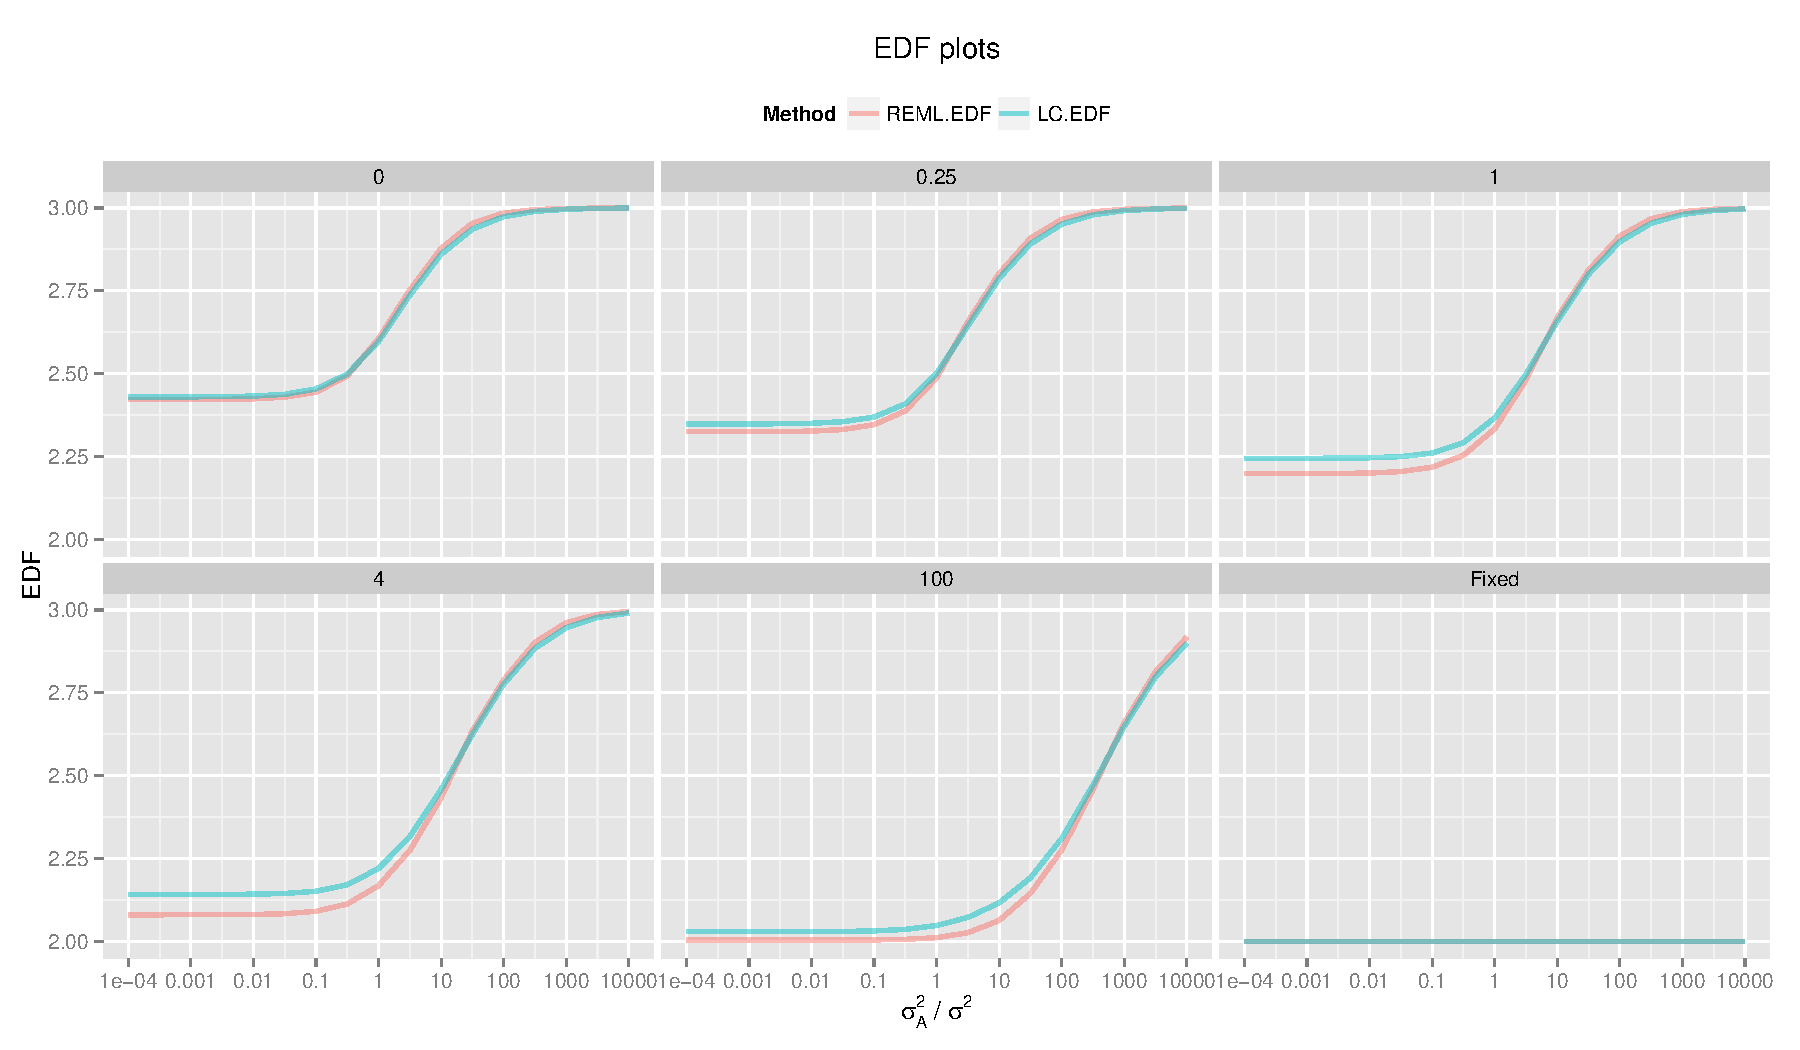
\includegraphics[width=1 \textwidth]{Graph/CRD232Tag4.pdf}
\caption{Plots of EDF from the negative VC are adjusted to zero.}
\label{fig:EDFadjusted}
\end{figure}

\begin{figure}[ht]
\centering
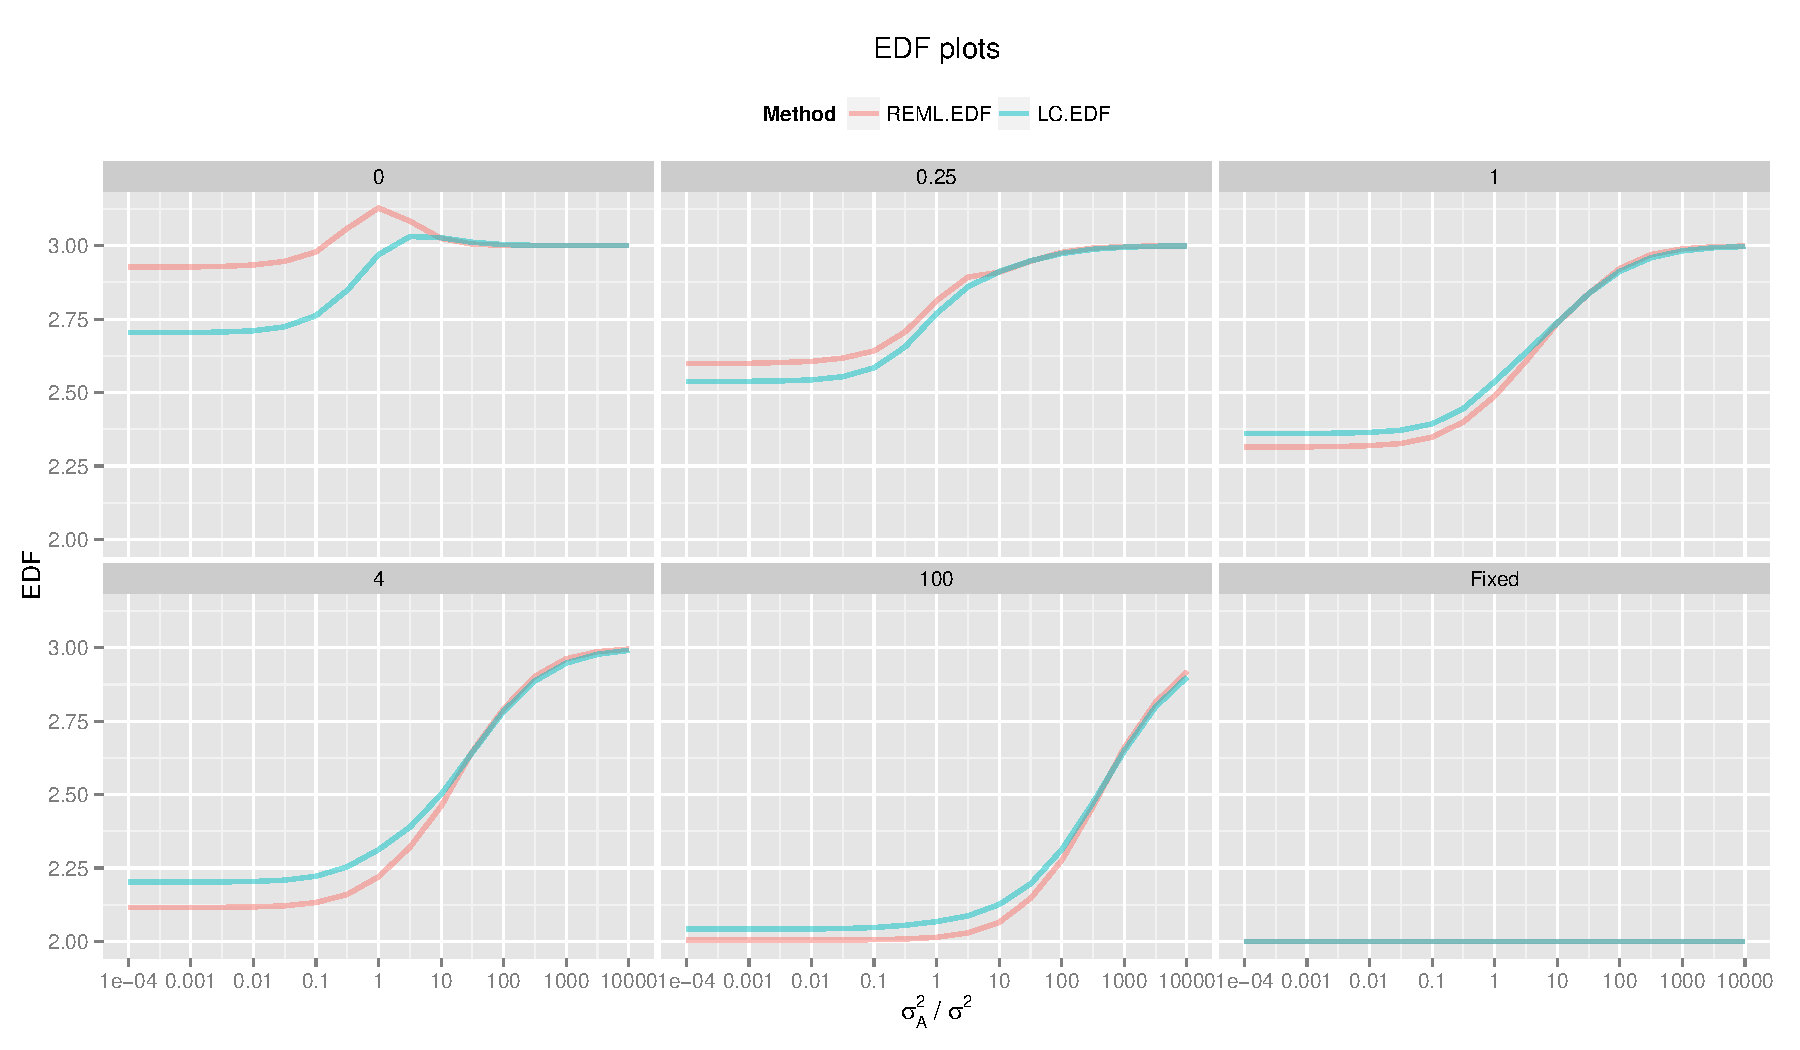
\includegraphics[width=1 \textwidth]{Graph/CRD232Tag4Unadjusted.pdf}
\caption{Plots of the EDF from the negative VC remain unadjusted.}
\label{fig:EDFunadjusted}
\end{figure}

From the EDF plots of the adjusted VC, the EDF are better when LC method is used. If the VC stays unadjusted, the EDF are only better when the both between runs and between animals VC estimates are low. The EDF from the adjusted VC are always bound in between 2 and 3, whereas the EDF from the unadjusted VC as high as 3.18 from using the REML method at $\sigma^2_R = 0$ and $\sigma^2_A = 1$. The EDF from the unadjusted VC are always higher than EDF from using adjusted VC. This is because once the negative VC adjusted to zero, the estimated VC can be higher than expected. The EDF can then be computed lower than expected. However, in theory, the EDF for this experiment should not be greater than 3 which is the maximum amount of DF associated with Between Animals stratum from the Phase 1 experiment. 

\subsection{Power analysis using the EDF}
Having the EDF computed, it can be used for conducting the tests for the treatment effects. The residual MS also needs re-calculated using the VC estimated from either REML or LC method. Given that the residual DF increases from 2 to 3, the critical F-ratio at significance level of 0.05 decreases from 18.51282 to 10.12796; hence, the power of the F-test should increase greatly.  

From the EDF plot, it shows that the EDF increases as the variation of between animals increases. Recall the power analysis from previous chapter where the two different designs with different residual DF were compared, the power of the test decreases as the variation of between animals increases. Thus, the main question here is that while the inflation of EDF causes by the inflation of the between animals variation and reduction of the between runs variation; is the estimated EDF high enough to increase the test power while the between animals variation also increases. 

Since the test for the treatment effects need to be conducted, the treatment effects need to be included into the simulated datasets. Hence, unlike the previous EDF plot generated from the simulated MS from the chi-square distribution, the following power plots are obtained from the simulated dataset generated from the normal distribution. The simulated datasets are generated with the true treatment mean groups of 0 and 4 and the true VC are remain the same as before. The highest EDF between the LC and REML methods are used for conducting the test for the treatment effects. The residual MS also needs to be adjusted based on the VC estimates from the method that generates the highest EDF. The powers of the F-test is compared between using the EDF with adjusted residual MS and using the original DF of 2 with residual MS from the ANOVA table. Moreover, the power plots based on the EDF computed from the adjusted VC and unadjusted VC are presented in Figure~\ref{fig:PowerAdjusted} and ~\ref{fig:PowerUnadjusted}, respectively.

\begin{figure}[ht]
\centering
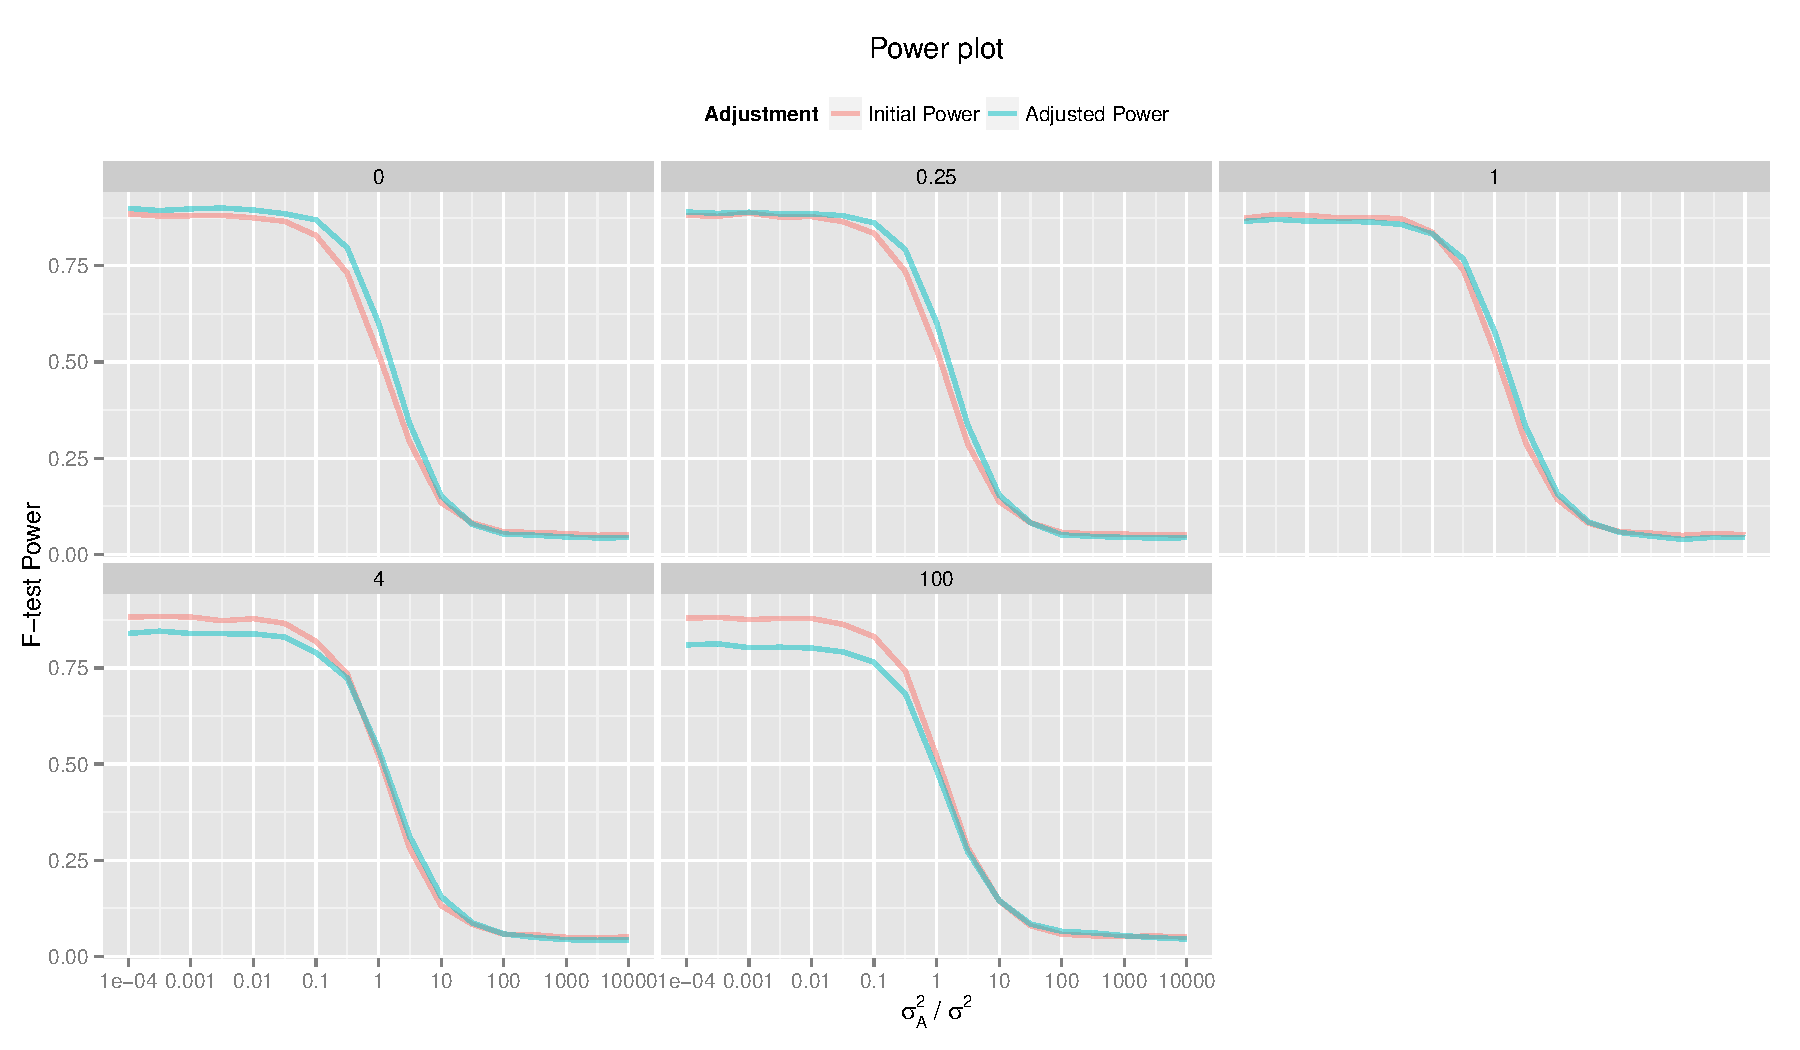
\includegraphics[width=1 \textwidth]{Graph/adjustZeroPowerEDF.pdf}
\caption{Plots of the F-test power from EDF of adjusted VC.}
\label{fig:PowerAdjusted}
\end{figure}

When the negative VC are adjusted to zero, the F-test power can be greater when using original DF of 2 with residual MS from the ANOVA table when the low $\sigma_A^2$ and high $\sigma_R^2$. 

\begin{figure}[ht]
\centering
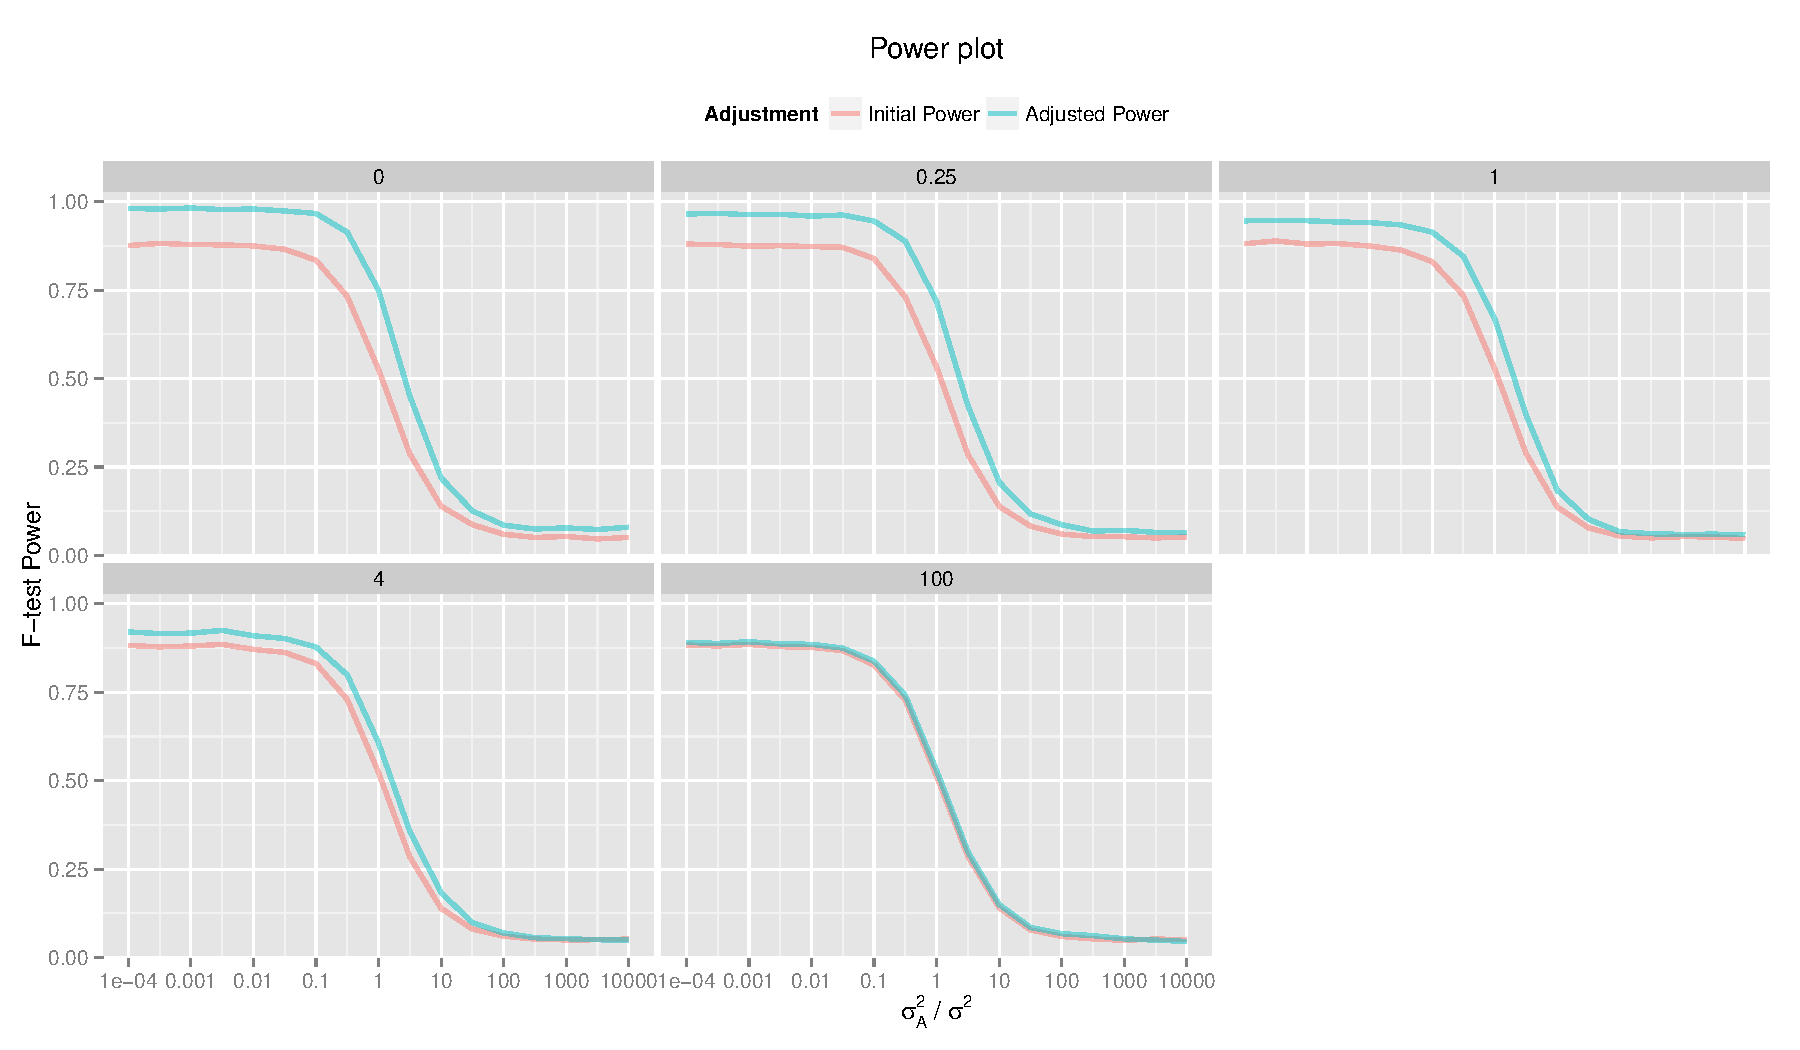
\includegraphics[width=1 \textwidth]{Graph/remainNegPowerEDF.pdf}
\caption{Plots of the F-test power from EDF of unadjusted VC.}
\label{fig:PowerUnadjusted}
\end{figure}

When the negative VC are stays unadjusted, the F-test power are better than when the negative VC are adjusted to zero. This is because the negative VC can lead to higher EDF, as shown in Figure~\ref{fig:EDFunadjusted}, as well as lower estimated residual MS; thus, the power of the F-test increases. 

In conclusion, using the adjusted VC is more accurate theoretically, because the EDF are always bounded within the expected range. However, the EDF can be screwed by the peak where estimated $\sigma_A^2$ and $\sigma_R^2$ are both zero. For more practical purposes, using the EDF with unadjusted VC can be better, because the mean of adjusted VC estimates are tend to be higher than the mean of adjusted VC estimates. Hence, the statistical power can be greatly increase as shown in Figure~\ref{fig:PowerUnadjusted}. However, negative VC estimates can cause the EDF to be much higher than expected; thus, the EDF will not be bounded within the expected range as shown from Figure~\ref{fig:EDFunadjusted}.
  
\section{Comparing the EDF when Phase 1 is CRD}
This section compares the EDF obtained from the two-phase optimal designs found where the Phase 1 experiment is arranged in CRD. The main focus is comparing between 4-plex and 8-plex experiments using the identical Phase 1 experiment. Three different cases are presented which shows that different sets of design parameters can be better using either 4-plex for 8-plex experiment.

\subsection{First CRD example}
The first example experiment to be compared is where Phase 1 experiment consists of $v = 2$, $r_b = 6$ and $r_t = 2$. The theoretical ANOVA tables from the optimal design where Phase 2 experiments use 4 tags are 8 tags are presented in Table~\ref{tab:ANOVAPhase1CRD11} and \ref{tab:ANOVAPhase1CRD12}, respectively. 
Based on these two theoretical ANOVA tables, the design with 4-plex is shown to be better, because this 4-plex experiment has both higher residual DF and treatment average efficiency factors than the 8-plex experiments for conducting the tests for the treatment effects. 

\begin{table}[ht]
\centering
 \caption{Theoretical ANOVA table from the Phase 1 experiment arrange in CRD with $v = 2$ and $r_b = 6$ and Phase 2 experiment uses 4 tags.}
 \begin{tabular}[t]{lrlll} 
 \toprule 
 \multicolumn{1}{l}{\textbf{Source of Variation}} & \multicolumn{1}{l}{\textbf{DF}} & \multicolumn{1}{l}{\textbf{EMS}}& \multicolumn{1}{l}{$\bm{E_{\gamma}}$}&\multicolumn{1}{l}{$\bm{E_{\tau}}$}\\ 
 \midrule 
 Between Runs &  &  & & \\ 
 \quad Between Animals & $2$ & $\sigma^2+2\sigma_{A}^2+4\sigma_{R}^2$ & & \\  \quad Within Animals & $3$ & $\sigma^2+4\sigma_{R}^2$ & & \\ \hline 
 Within Runs &  &  & & \\ 
 \quad Between Animals &  &  & & \\ 
 \quad \quad Tag & $1$ & $\sigma^2+2\sigma_{A}^2+6\theta_{\gamma}$ &$1$ & \\ 
 \quad \quad Treatment & $1$ & $\sigma^2+2\sigma_{A}^2+12\theta_{\tau}$ & & $1$\\ 
 \quad \quad Residual & $7$ & $\sigma^2+2\sigma_{A}^2$ & & \\ \hline 
 \quad Within Animals &  &  & & \\ 
 \quad \quad Tag & $2$ & $\sigma^2+6\theta_{\gamma}$ &$1$ & \\ 
 \quad \quad Residual & $7$ & $\sigma^2$ & & \\ 
 \bottomrule 
 \end{tabular} 
 \label{tab:ANOVAPhase1CRD11} 
\end{table} 

\begin{table}[ht]
\centering
 \caption{Theoretical ANOVA table from the Phase 1 experiment arrange in CRD with $v = 2$ and $r_b = 6$ and Phase 2 experiment uses 8 tags.}
 \begin{tabular}[t]{lrlll} 
 \toprule 
 \multicolumn{1}{l}{\textbf{Source of Variation}} & \multicolumn{1}{l}{\textbf{DF}} & \multicolumn{1}{l}{\textbf{EMS}}& \multicolumn{1}{l}{$\bm{E_{\gamma}}$}&\multicolumn{1}{l}{$\bm{E_{\tau}}$}\\ 
 \midrule 
 Between Runs &  &  & & \\ 
 \quad Between Animals & $1$ & $\sigma^2+2\sigma_{A}^2+8\sigma_{R}^2$ & & \\  \quad Within Animals & $1$ & $\sigma^2+8\sigma_{R}^2$ & & \\ \hline 
 Within Runs &  &  & & \\ 
 \quad Between Animals &  &  & & \\ 
 \quad \quad Tag & $3$ & $\sigma^2+2\sigma_{A}^2+3\theta_{\gamma}+ \frac{4}{3}\theta_{\tau}$ &$1$ & $\frac{1}{9}$\\ 
 \quad \quad Treatment & $1$ & $\sigma^2+2\sigma_{A}^2+\frac{32}{3}\theta_{\tau}$ & & $\frac{8}{9}$\\ 
 \quad \quad Residual & $6$ & $\sigma^2+2\sigma_{A}^2$ & & \\ \hline 
 \quad Within Animals &  &  & & \\ 
 \quad \quad Tag & $4$ & $\sigma^2+3\theta_{\gamma}$ &$1$ & \\ 
 \quad \quad Residual & $7$ & $\sigma^2$ & & \\ 
 \bottomrule 
 \end{tabular} 
 \label{tab:ANOVAPhase1CRD12} 
\end{table} 

The plots of EDF are expressed in Figure~\ref{fig:compare48CRD1}, which also shows the EDF from the 4-plex experiment are always higher than the EDF of the 8-plex experiment when the Phase 1 experiment is CRD with $v = 2$, $r_b = 6$ and $r_t = 2$. The EDF are at least 1 DF higher when the VC of between animals is low. However, the VC of between animals increases, the EDF can be as high as 2 DF. 

\begin{figure}[ht]
\centering
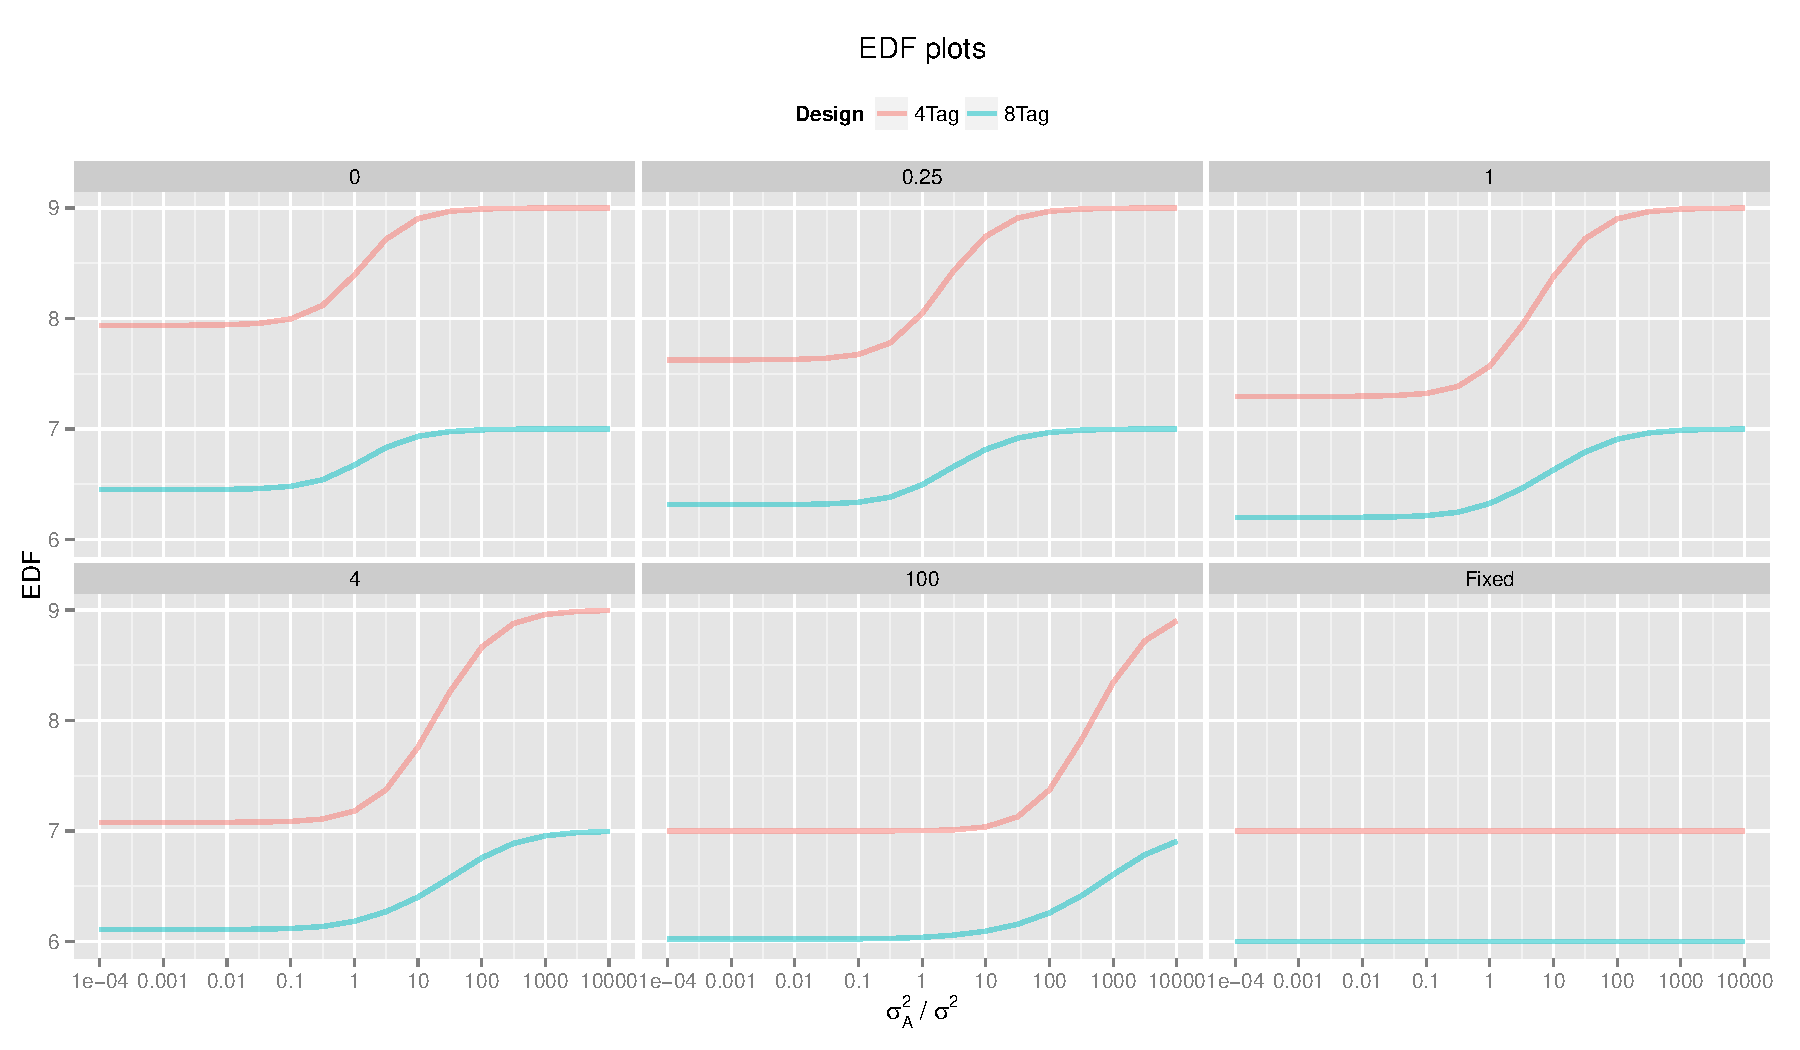
\includegraphics[width=1 \textwidth]{Graph/CRD262Tag4vsTag8.pdf}
\caption{Plots of EDF for the experiments with $v = 2, r_b = 6$ comparing between 4-plex and 8-plex systems.}
\label{fig:compare48CRD1}
\end{figure}


This case is very typical when the Phase 1 experiment is CRD. This is because the Between Animals stratum always have 1 DF associated with tag effects for the 4-plex experiments, whereas the 8-plex experiments generally have 3 DF associated with tag effect in the Between Animals stratum. Hence, the EDF from the experiments with 4 tags can have at most 2 DF higher to the experiments with 8 tags for estimating the residual MS in the Between Animals strata in Between and Within Runs strata. Therefore, for general cases, the 4-plex experiments is better to the 8-plex experiments.

%When the comparisons can be done, the experiment using the 4-plex system tend to have higher EDF, because the Between Animals DF that are confounded with tag effects is lesser; thus as the between animals variation become much larger than the variation between runs, the EDF will also increases. 

\subsection{Second CRD example}
The second experiment considers the experiment with $v = 4, r_b = 6$ and $r_t = 2$. The theoretical ANOVA tables from the optimal design where Phase 2 experiments use 4 tags are 8 tags are presented in Table~\ref{tab:ANOVAPhase1CRD21} and \ref{tab:ANOVAPhase1CRD22}, respectively. 
Based on these two theoretical ANOVA tables, the design with 8 tags is shown to be better, because this 8-plex experiment has higher residual DF than the 4-plex experiments for conducting the tests for the treatment effects. However, the treatment average efficiency factors from the designs with 8-plex experiment is $0.9623$ which is slightly lower than the treatment average efficiency factors for the 4-plex experiment of $100\%$.  

\begin{table}[ht]
\centering
 \caption{Theoretical ANOVA table from the Phase 1 experiment arrange in CRD with $v = 4$ and $r_b = 6$ and Phase 2 experiment uses 4 tags.}
 \begin{tabular}[t]{lrlll} 
 \toprule 
 \multicolumn{1}{l}{\textbf{Source of Variation}} & \multicolumn{1}{l}{\textbf{DF}} & \multicolumn{1}{l}{\textbf{EMS}}& \multicolumn{1}{l}{$\bm{E_{\gamma}}$}&\multicolumn{1}{l}{$\bm{E_{\tau}}$}\\ 
 \midrule 
 Between Runs &  &  & & \\ 
 \quad Between Animals & $5$ & $\sigma^2+2\sigma_{A}^2+4\sigma_{R}^2$ & & \\  \quad Within Animals & $6$ & $\sigma^2+4\sigma_{R}^2$ & & \\ \hline 
 Within Runs &  &  & & \\ 
 \quad Between Animals &  &  & & \\ 
 \quad \quad Tag & $1$ & $\sigma^2+2\sigma_{A}^2+12\theta_{\gamma}$ &$1$ & \\ 
 \quad \quad Treatment & $3$ & $\sigma^2+2\sigma_{A}^2+12\theta_{\tau}$ & & $1$\\ 
 \quad \quad Residual & $14$ & $\sigma^2+2\sigma_{A}^2$ & & \\ \hline 
 \quad Within Animals &  &  & & \\ 
 \quad \quad Tag & $2$ & $\sigma^2+12\theta_{\gamma}$ &$1$ & \\ 
 \quad \quad Residual & $16$ & $\sigma^2$ & & \\ 
 \bottomrule 
 \end{tabular} 
 \label{tab:ANOVAPhase1CRD21} 
\end{table} 

\begin{table}[ht]
\centering
 \caption{Theoretical ANOVA table from the Phase 1 experiment arrange in CRD with $v = 4$ and $r_b = 6$ and Phase 2 experiment uses 8 tags.}
 \begin{tabular}[t]{lrlll} 
 \toprule 
 \multicolumn{1}{l}{\textbf{Source of Variation}} & \multicolumn{1}{l}{\textbf{DF}} & \multicolumn{1}{l}{\textbf{EMS}}& \multicolumn{1}{l}{$\bm{E_{\gamma}}$}&\multicolumn{1}{l}{$\bm{E_{\tau}}$}\\ 
 \midrule 
 Between Runs &  &  & & \\ 
 \quad Between Animals & $2$ & $\sigma^2+2\sigma_{A}^2+8\sigma_{R}^2$ & & \\  \quad Within Animals & $3$ & $\sigma^2+8\sigma_{R}^2$ & & \\ \hline 
 Within Runs &  &  & & \\ 
 \quad Between Animals &  &  & & \\ 
 \quad \quad Tag & $3$ & $\sigma^2+2\sigma_{A}^2+6\theta_{\gamma}+ \frac{2}{3}\theta_{\tau}$ &$1$ & $\frac{1}{18}$\\ 
 \quad \quad Treatment & $3$ & $\sigma^2+2\sigma_{A}^2+ \frac{612}{53}\theta_{\tau}$ & & $\frac{51}{53}$\\ 
 \quad \quad Residual & $15$ & $\sigma^2+2\sigma_{A}^2$ & & \\ \hline 
 \quad Within Animals &  &  & & \\ 
 \quad \quad Tag & $4$ & $\sigma^2+6\theta_{\gamma}$ &$1$ & \\ 
 \quad \quad Residual & $17$ & $\sigma^2$ & & \\ 
 \bottomrule 
 \end{tabular} 
 \label{tab:ANOVAPhase1CRD22} 
\end{table} 

The plot of EDF can be expressed in Figure~\ref{fig:compare44CRD}. The EDF from the 4-plex experiments are always higher than the 8-plex experiments when the between runs VC is zero. Otherwise, the EDF from the 8-plex experiment can be higher than the 4-plex experiment with the low between animal VC. However, as the between animals VC increases, the EDF of 4-plex experiments become better than the experiment with 8 tags. Thus, the 8-plex experiments are only better than 4-plex experiments with low between animals VC and high between runs VC estimates.

\begin{figure}[ht]
\centering
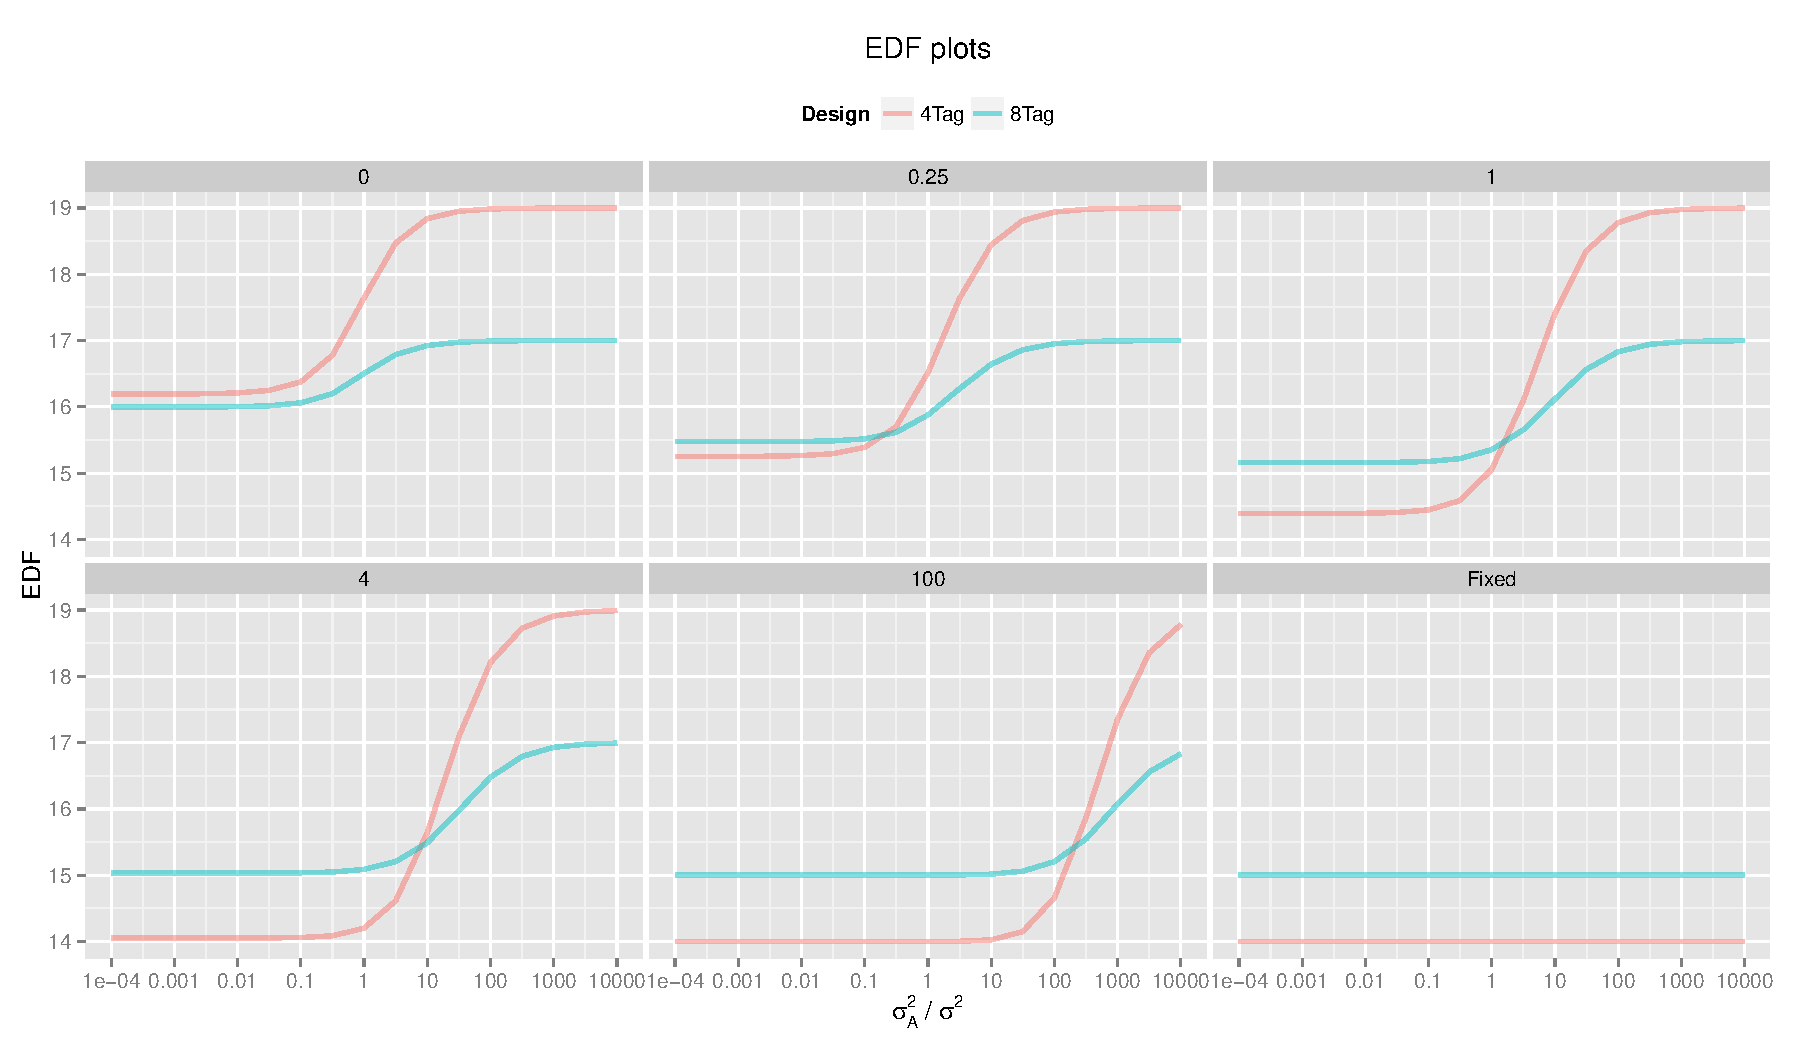
\includegraphics[width=1 \textwidth]{Graph/CRD462Tag4vsTag8.pdf}
\caption{Plots of EDF for the experiments with $v = 4, r_b = 6$ comparing between 4-plex and 8-plex systems.}
\label{fig:compare44CRD}
\end{figure}

This type of situation occurs when the $r_b$ is high in the Phase 1 experiment. Due to the disconnectedness in the allocation of animals to runs, some DF associated with Between Animals stratum can be in the Between Runs stratum. As the $r_b$ is increases, the 4-plex experiments will have more DF associated with animals in the Between Runs stratum than the 8-plex experiment. This is because the each run of the 4-plex experiment can only measures up to 4 samples. 

However, as the biological replicate increases, the residual DF will also increase. For this example with $v = 4, r_b = 6$ and $r_t = 2$., the critical F-ratio with the significance level at 0.05 from $(3,19)$ DF and $(3,14)$ are  3.12735 and 3.343889. Thus, the power of the F-test comparing between these two designs should not be very different. Therefore, these two designs should be  equally effective under different between runs and between animals VC.

\subsection{Third CRD example}
The third experiment considers the experiment with $v = 8, r_b = 2$ and $r_t = 2$. The theoretical ANOVA tables from the optimal design where Phase 2 experiments use 4 tags are 8 tags are presented in Table~\ref{tab:ANOVAPhaseCRD31} and \ref{tab:ANOVAPhaseCRD32}, respectively. 
Based on these two theoretical ANOVA tables, these two designs are equally effective in both higher residual DF and treatment average efficiency factors. 

\begin{table}[ht]
\centering
 \caption{Theoretical ANOVA table from the Phase 1 experiment arrange in CRD with $v = 8$ and $r_b = 2$ and Phase 2 experiment uses 4 tags.}
 \begin{tabular}[t]{lrlll} 
 \toprule 
 \multicolumn{1}{l}{\textbf{Source of Variation}} & \multicolumn{1}{l}{\textbf{DF}} & \multicolumn{1}{l}{\textbf{EMS}}& \multicolumn{1}{l}{$\bm{E_{\gamma}}$}&\multicolumn{1}{l}{$\bm{E_{\tau}}$}\\ 
 \midrule 
 Between Runs &  &  & & \\ 
 \quad Between Animals &  &  & & \\ 
 \quad \quad Treatment & $3$ & $\sigma^2+2\sigma_{A}^2+4\sigma_{R}^2+\frac{6}{5}\theta_{\tau}$ & & $\frac{3}{10}$\\ 
 \quad Within Animals & $4$ & $\sigma^2+4\sigma_{R}^2$ & & \\ \hline 
 Within Run &  &  & & \\ 
 \quad Between Animals &  &  & & \\ 
 \quad \quad Tag & $1$ & $\sigma^2+2\sigma_{A}^2+8\theta_{\gamma}$ &$1$ & \\ 
 \quad \quad Treatment & $7$ & $\sigma^2+2\sigma_{A}^2+\frac{42}{13}\theta_{\tau}$ & & $\frac{21}{26}$\\ 
 \quad \quad Residual & $4$ & $\sigma^2+2\sigma_{A}^2$ & & \\ \hline 
 \quad Within Animals &  &  & & \\ 
 \quad \quad Tag & $2$ & $\sigma^2+8\theta_{\gamma}$ &$1$ & \\ 
 \quad \quad Residual & $10$ & $\sigma^2$ & & \\ 
 \bottomrule 
 \end{tabular} 
 \label{tab:ANOVAPhaseCRD31} 
\end{table} 

\begin{table}[ht]
\centering
 \caption{Theoretical ANOVA table from the Phase 1 experiment arrange in CRD with $v = 8$ and $r_b = 2$ and Phase 2 experiment uses 8 tags.}
 \begin{tabular}[t]{lrlll} 
 \toprule 
 \multicolumn{1}{l}{\textbf{Source of Variation}} & \multicolumn{1}{l}{\textbf{DF}} & \multicolumn{1}{l}{\textbf{EMS}}& \multicolumn{1}{l}{$\bm{E_{\gamma}}$}&\multicolumn{1}{l}{$\bm{E_{\tau}}$}\\ 
 \midrule 
 Between Runs &  &  & & \\ 
 \quad Between Animals & $1$ & $\sigma^2+2\sigma_{A}^2+8\sigma_{R}^2$ & & \\ 
 \quad Within Animals & $2$ & $\sigma^2+8\sigma_{R}^2$ & & \\ \hline 
 Within Runs &  &  & & \\ 
 \quad Between Animals &  &  & & \\ 
 \quad \quad Tag & $3$ & $\sigma^2+2\sigma_{A}^2+4\theta_{\gamma}+\frac{6}{5}\theta_{\tau}$ &$1$ & $\frac{3}{10}$\\ 
 \quad \quad Treatment & $7$ & $\sigma^2+2\sigma_{A}^2+\frac{42}{13}\theta_{\tau}$ & & $\frac{21}{26}$\\ 
 \quad \quad Residual & $4$ & $\sigma^2+2\sigma_{A}^2$ & & \\ \hline 
 \quad Within Animals &  &  & & \\ 
 \quad \quad Tag & $4$ & $\sigma^2+4\theta_{\gamma}$ &$1$ & \\ 
 \quad \quad Residual & $10$ & $\sigma^2$ & & \\ 
 \bottomrule 
 \end{tabular} 
 \label{tab:ANOVAPhaseCRD32} 
\end{table} 

The plot of EDF can be expressed in Figure~\ref{fig:compare82CRD}, which shows the EDF from the 8-plex experiment are higher than the EDF of the 4-plex experiment, especially when the VC estimates are low for between runs and high for between animals. The EDF can be the same between the two designs with low between animals VC and high between runs VC. Therefore, when the Phase 1 experiment is CRD with $v = 5$, $r_b = 2$ and $r_t = 2$, the 8-plex experiment is preferred.

\begin{figure}[ht]
\centering
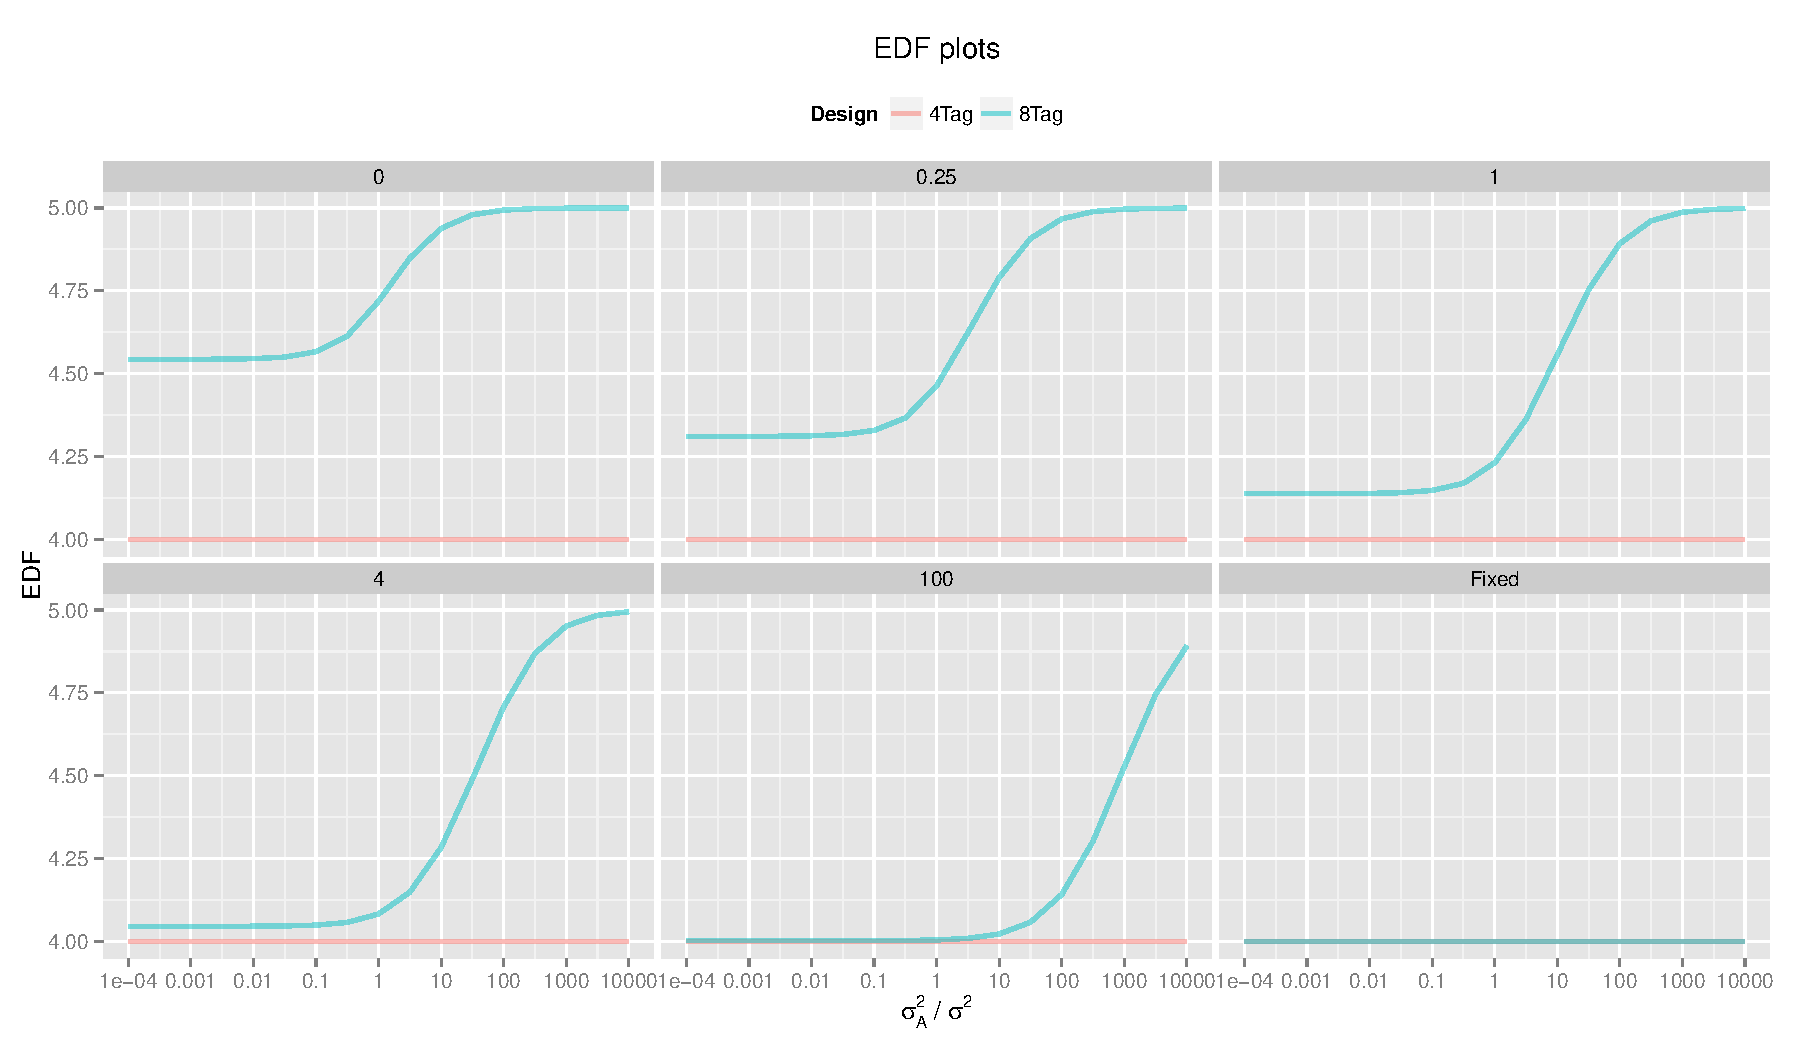
\includegraphics[width=1 \textwidth]{Graph/CRD822Tag4vsTag8.pdf}
\caption{Plots of EDF for the experiments with $v = 8, r_b = 2$ comparing between 4-plex and 8-plex systems.}
\label{fig:compare82CRD}
\end{figure}

This example shows that the 8-plex experiment is only always better when comparing between 8 treatments in the Phase 1 experiment. As shown from the theoretical ANOVA table in Table~\ref{tab:ANOVAPhaseCRD31}, some treatment information are in the Between Runs stratum which also confounded all 3 DF associated with Between Animals stratum. Thus, it is not possible to recover these 3 DF using the method presented in this chapter. Therefore, EDF for the experiment with 4-plex experiment stays at 4 with different VC estimates. As for the experiment with 8 tags, from the theoretical ANOVA table in Table~\ref{tab:ANOVAPhaseCRD32}, the treatments are not confounded with runs; hence, the 1 DF associated with Between Animals stratum in the Between Runs can be recovered with high between animals VC and low between runs VC. Therefore, the 8-plex experiment is better for the experiment of comparing between 8 treatments.  

To summarise, when the Phase 1 experiment is CRD, using the 4-plex system is generally preferable with low number of biological replicates. As the number of  biological replicates increases, the 8-plex system can have higher EDF than 4-plex system with low between animals VC and high between runs VC. However, the power of F-tests should not be very different, since the critical F-ratio between the two designs are very similar. For the time and budget issues, the 8-plex system should be preferred, because it can measure more samples in the same run. When comparing between 8 treatment, the 8-plex experiment should always be used, because the treatment are orthogonal to runs which maximised the information of animals. 

\section{Compare the EDF where Phase 1 experiment is RBD}
\label{sec:expRBD}
This section compares the EDF obtained from the two-phase optimal designs found where the Phase 1 experiment is arranged in RBD. The Phase 1 experiment uses cages as the blocking for set of the animals. Having this cage component, recall from the Chapter for searching for optimal design, the initial designs can be have cage confounded more with tags or with runs. As well as comparing between using these two initial designs, the designs from 4-plex and 8-plex experiments can also be compared. An example where Phase 1 experiment is arranged in RBD illustrate how the allocation of cages to runs and tags can also affect the EDF with different VC estimates.  

\subsection{The RBD example} 
The example experiment to be compared is where Phase 1 experiment consists of $v = 4$, $r_b = 4, n_B  = 4$ and $r_t = 2$. There are four different two-phase designs can compared using the identical Phase 1 experiment. The theoretical ANOVA tables for each of these four designs are presented in Table~\ref{tab:ANOVAPhase1RBD1}, \ref{tab:ANOVAPhase1RBD2}, \ref{tab:ANOVAPhase1RBD3} and \ref{tab:ANOVAPhase1RBD4}. Based on these four theoretical ANOVA tables, Table~\ref{tab:ANOVAPhase1RBD1} and \ref{tab:ANOVAPhase1RBD4} are appeared to performed equally well with the highest residual DF of 8 and $100\%$ of the treatment information in the Between Animals Within Cages Within Runs stratum. However, as shown from the second CRD example, the EDF may be better in the different design with the different VC estimates. Hence, the EDF need to be assess from these four designs. 

\begin{table}[ht]
\centering
 \caption{Theoretical ANOVA table from the Phase 1 is RBD with $v = 4$ and $r_b = 4$ and Phase 2 experiment uses 4 tags with the initial design that cage is confounded more with runs.}
 \begin{tabular}[t]{lrlll} 
 \toprule 
 \multicolumn{1}{l}{\textbf{Source of Variation}} & \multicolumn{1}{l}{\textbf{DF}} & \multicolumn{1}{l}{\textbf{EMS}}& \multicolumn{1}{l}{$\bm{E_{\gamma}}$}&\multicolumn{1}{l}{$\bm{E_{\tau}}$}\\ 
 \midrule 
 Between Runs &  &  & & \\ 
 \quad Between Cages & $3$ & $\sigma^2+2\sigma_{A}^2+8\sigma_{B}^2+4\sigma_{R}^2$ & & \\  
 \quad Within Animals Within Cages & $4$ & $\sigma^2+4\sigma_{R}^2$ & & \\ \hline 
 Within Runs &  &  & & \\ 
 \quad Between Animals Within Cages &  &  & & \\ 
 \quad \quad Tag & $1$ & $\sigma^2+2\sigma_{A}^2+8\theta_{\gamma}$ &$1$ & \\ 
 \quad \quad Treatment & $3$ & $\sigma^2+2\sigma_{A}^2+8\theta_{\tau}$ & & $1$\\ 
 \quad \quad Residual & $8$ & $\sigma^2+2\sigma_{A}^2$ & & \\ \hline 
 \quad Within Animals Within Cages &  &  & & \\ 
 \quad \quad Tag & $2$ & $\sigma^2+8\theta_{\gamma}$ &$1$ & \\ 
 \quad \quad Residual & $10$ & $\sigma^2$ & & \\ 
 \bottomrule 
 \end{tabular} 
 \label{tab:ANOVAPhase1RBD1} 
\end{table} 

\begin{table}[ht]
\centering
 \caption{Theoretical ANOVA table from the Phase 1 is RBD with $v = 4$ and $r_b = 4$ and Phase 2 experiment uses 4 tags with the initial design that cage is confounded more with tags.}
 \begin{tabular}[t]{lrlll} 
 \toprule 
 \multicolumn{1}{l}{\textbf{Source of Variation}} & \multicolumn{1}{l}{\textbf{DF}} & \multicolumn{1}{l}{\textbf{EMS}}& \multicolumn{1}{l}{$\bm{E_{\gamma}}$}&\multicolumn{1}{l}{$\bm{E_{\tau}}$}\\ 
 \midrule 
 Between Runs &  &  & & \\ 
 \quad Between Cages & $1$ & $\sigma^2+2\sigma_{A}^2+8\sigma_{B}^2+4\sigma_{R}^2$ & & \\  
 \quad Between Animals Within Cages & $2$ & $\sigma^2+2\sigma_{A}^2+4\sigma_{R}^2$ & & \\  
 \quad Within Animals Within Cages & $4$ & $\sigma^2+4\sigma_{R}^2$ & & \\ \hline 
 Within Runs &  &  & & \\ 
 \quad Between Cages &  &  & & \\ 
 \quad \quad Tag & $1$ & $\sigma^2+2\sigma_{A}^2+8\sigma_{B}^2+8\theta_{\gamma}$ &$1$ & \\ 
 \quad \quad Residual & $1$ & $\sigma^2+2\sigma_{A}^2+8\sigma_{B}^2$ & & \\ \hline 
 \quad Between Animals Within Cages &  &  & & \\ 
 \quad \quad Treatment & $3$ & $\sigma^2+2\sigma_{A}^2+8\theta_{\tau}$ & & $1$\\ 
 \quad \quad Residual & $7$ & $\sigma^2+2\sigma_{A}^2$ & & \\ \hline 
 \quad Within Animals Within Cages &  &  & & \\ 
 \quad \quad Tag & $2$ & $\sigma^2+8\theta_{\gamma}$ &$1$ & \\ 
 \quad \quad Residual & $10$ & $\sigma^2$ & & \\ 
 \bottomrule 
 \end{tabular} 
 \label{tab:ANOVAPhase1RBD2} 
\end{table} 


\begin{table}[ht]
\centering
 \caption{Theoretical ANOVA table from the Phase 1 is RBD with $v = 4$ and $r_b = 4$ and Phase 2 experiment uses 8 tags with the initial design that cage is confounded more with runs.}
 \begin{tabular}[t]{lrlll} 
 \toprule 
 \multicolumn{1}{l}{\textbf{Source of Variation}} & \multicolumn{1}{l}{\textbf{DF}} & \multicolumn{1}{l}{\textbf{EMS}}& \multicolumn{1}{l}{$\bm{E_{\gamma}}$}&\multicolumn{1}{l}{$\bm{E_{\tau}}$}\\ 
 \midrule 
 Between Runs &  &  & & \\ 
 \quad Between Cages & $1$ & $\sigma^2+2\sigma_{A}^2+8\sigma_{B}^2+8\sigma_{R}^2$ & & \\  
 \quad Within Animals Within Cages & $2$ & $\sigma^2+8\sigma_{R}^2$ & & \\ \hline 
 Within Runs &  &  & & \\ 
 \quad Between Cages &  &  & & \\ 
 \quad \quad Tag & $1$ & $\sigma^2+2\sigma_{A}^2+8\sigma_{B}^2+4\theta_{\gamma}$ &$1$ & \\ 
 \quad \quad Residual & $1$ & $\sigma^2+2\sigma_{A}^2+8\sigma_{B}^2$ & & \\ \hline 
 \quad Between Animals Within Cages &  &  & & \\ 
 \quad \quad Tag & $2$ & $\sigma^2+2\sigma_{A}^2+4\theta_{\gamma}$ &$1$ & \\ 
 \quad \quad Treatment & $3$ & $\sigma^2+2\sigma_{A}^2+8\theta_{\tau}$ & & $1$\\ 
 \quad \quad Residual & $7$ & $\sigma^2+2\sigma_{A}^2$ & & \\ \hline 
 \quad Within Animals Within Cages &  &  & & \\ 
 \quad \quad Tag & $4$ & $\sigma^2+4\theta_{\gamma}$ &$1$ & \\ 
 \quad \quad Residual & $10$ & $\sigma^2$ & & \\ 
 \bottomrule 
 \end{tabular} 
 \label{tab:ANOVAPhase1RBD3} 
\end{table} 

\begin{table}[ht]
\centering
 \caption{Theoretical ANOVA table from the Phase 1 is RBD with $v = 4$ and $r_b = 4$ and Phase 2 experiment uses 8 tags with the initial design that cage is confounded more with tags.}
 \begin{tabular}[t]{lrlll} 
 \toprule 
 \multicolumn{1}{l}{\textbf{Source of Variation}} & \multicolumn{1}{l}{\textbf{DF}} & \multicolumn{1}{l}{\textbf{EMS}}& \multicolumn{1}{l}{$\bm{E_{\gamma}}$}&\multicolumn{1}{l}{$\bm{E_{\tau}}$}\\ 
 \midrule 
 Between Runs &  &  & & \\ 
 \quad Between Animals Within Cages & $1$ & $\sigma^2+2\sigma_{A}^2+8\sigma_{R}^2$ & & \\ 
 \quad Within Animals Within Cages & $2$ & $\sigma^2+8\sigma_{R}^2$ & & \\ \hline 
 Within Runs &  &  & & \\ 
 \quad Between Cages &  &  & & \\ 
 \quad \quad Tag & $3$ & $\sigma^2+2\sigma_{A}^2+8\sigma_{B}^2+4\theta_{\gamma}$ &$1$ & \\ \hline 
 \quad Between Animals Within Cages &  &  & & \\ 
 \quad \quad Treatment & $3$ & $\sigma^2+2\sigma_{A}^2+8\theta_{\tau}$ & & $1$\\ 
 \quad \quad Residual & $8$ & $\sigma^2+2\sigma_{A}^2$ & & \\ \hline 
 \quad Within Animals Within Cages &  &  & & \\ 
 \quad \quad Tag & $4$ & $\sigma^2+4\theta_{\gamma}$ &$1$ & \\ 
 \quad \quad Residual & $10$ & $\sigma^2$ & & \\ 
 \bottomrule 
 \end{tabular} 
 \label{tab:ANOVAPhase1RBD4} 
\end{table} 

The first comparison of the EDF is between the two different initial designs using the 4-plex experiments. The plots of EDF are presented in Figure~\ref{fig:RBD442Tag4EDF}. The design from the where the cages is is confounded more with runs is presented by the pink line which the EDF are always 8. This situation can be explain by the theoretical ANOVA table in {tab:ANOVAPhase1RBD1}, where the Between Runs stratum does not contain the Between Animals Within Cages stratum. Another way to explain it is that the between VC estimates can only be derived from the Within Runs stratum. Back to Figure~\ref{fig:RBD442Tag4EDF}, the remaining 6 colours represents the EDF with different VC of between cages, which shows the between cages VC can only affect the EDF when the between animals VC is small.  

\begin{figure}[ht]
\centering
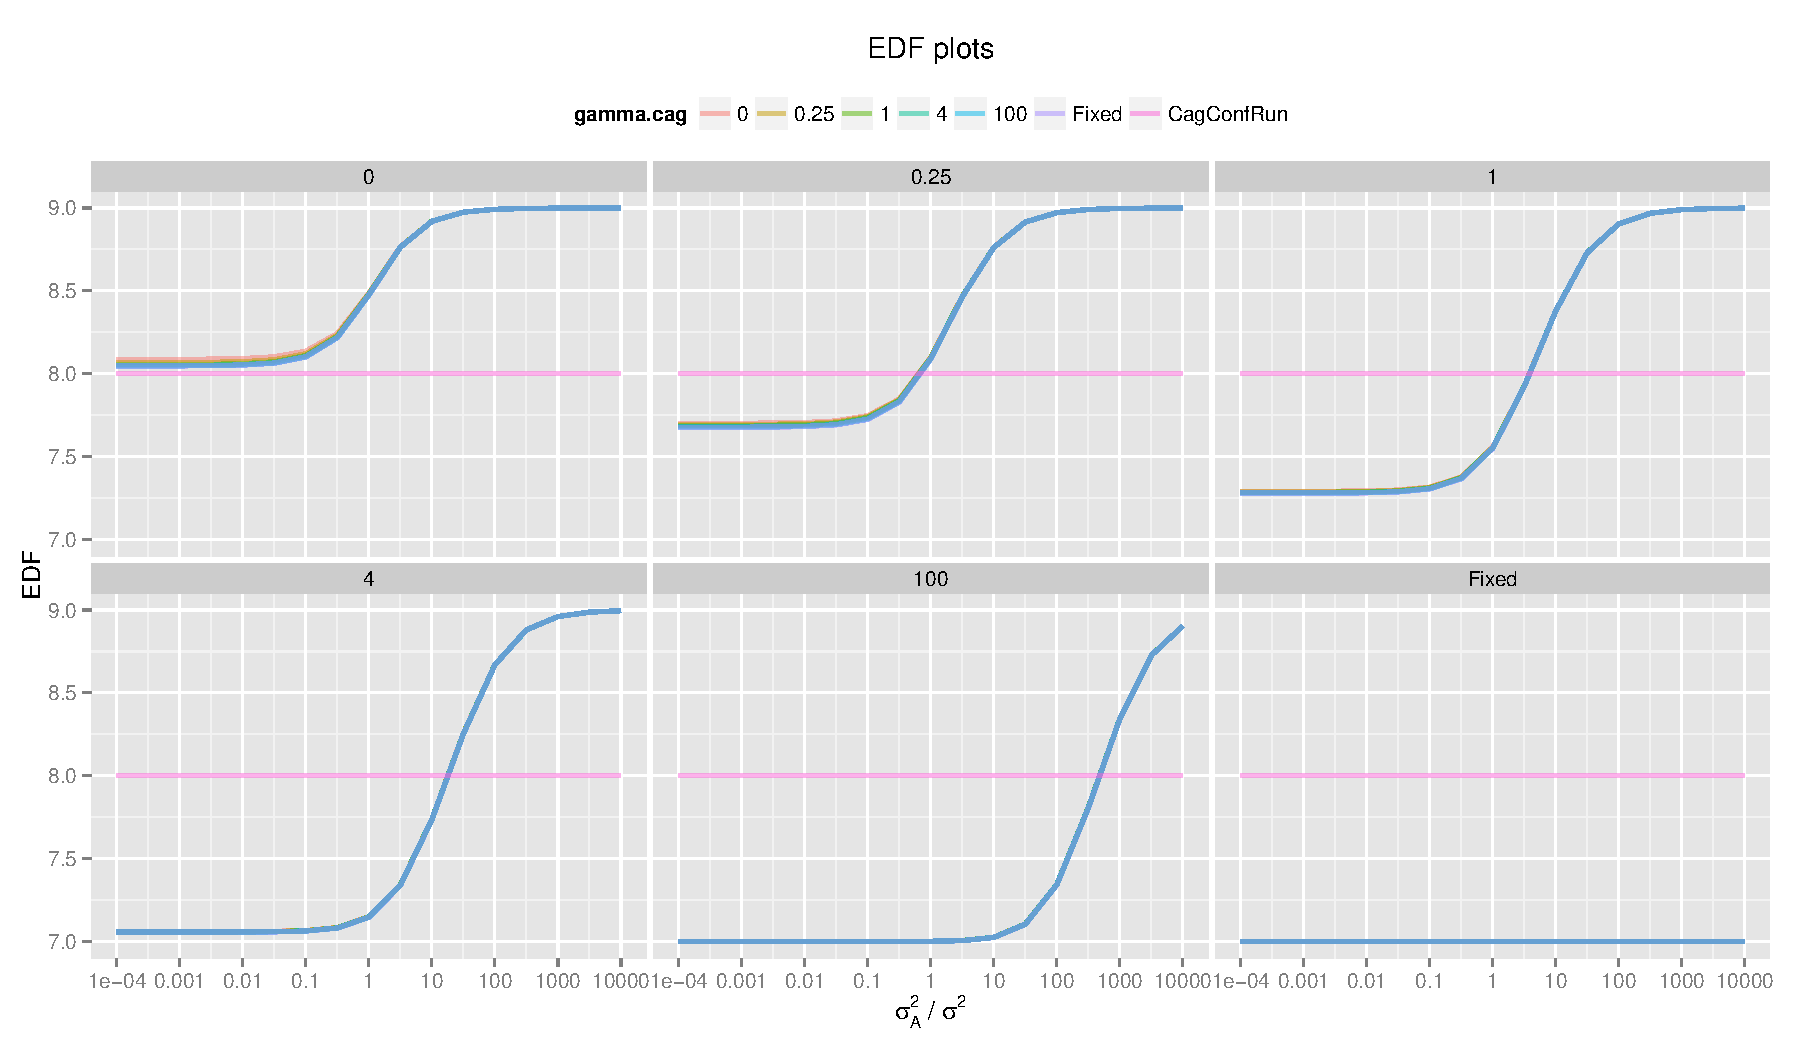
\includegraphics[width=1 \textwidth]{Graph/RBD442Tag4EDF.pdf}
\caption{Plots of EDF for the RBD experiments with $v = 4, r_b = 4$ and $n_B = 4$ comparing between different between cages VC estimates with the initial design where cages is confounded more with tags and the initial design where cages is confounded more with runs with Phase 2 experiment uses 4 tags.}
\label{fig:RBD442Tag4EDF}
\end{figure}

Figure~\ref{fig:RBD442Tag4EDFRun0} only focuses on the when the between runs VC is zero of Figure~\ref{fig:RBD442Tag4EDF}. Notice EDF is the greatest when the between cages VC is zero; however, the differences of EDF from different between cages VC too small to affect the power of the test.    

\begin{figure}[ht]
\centering
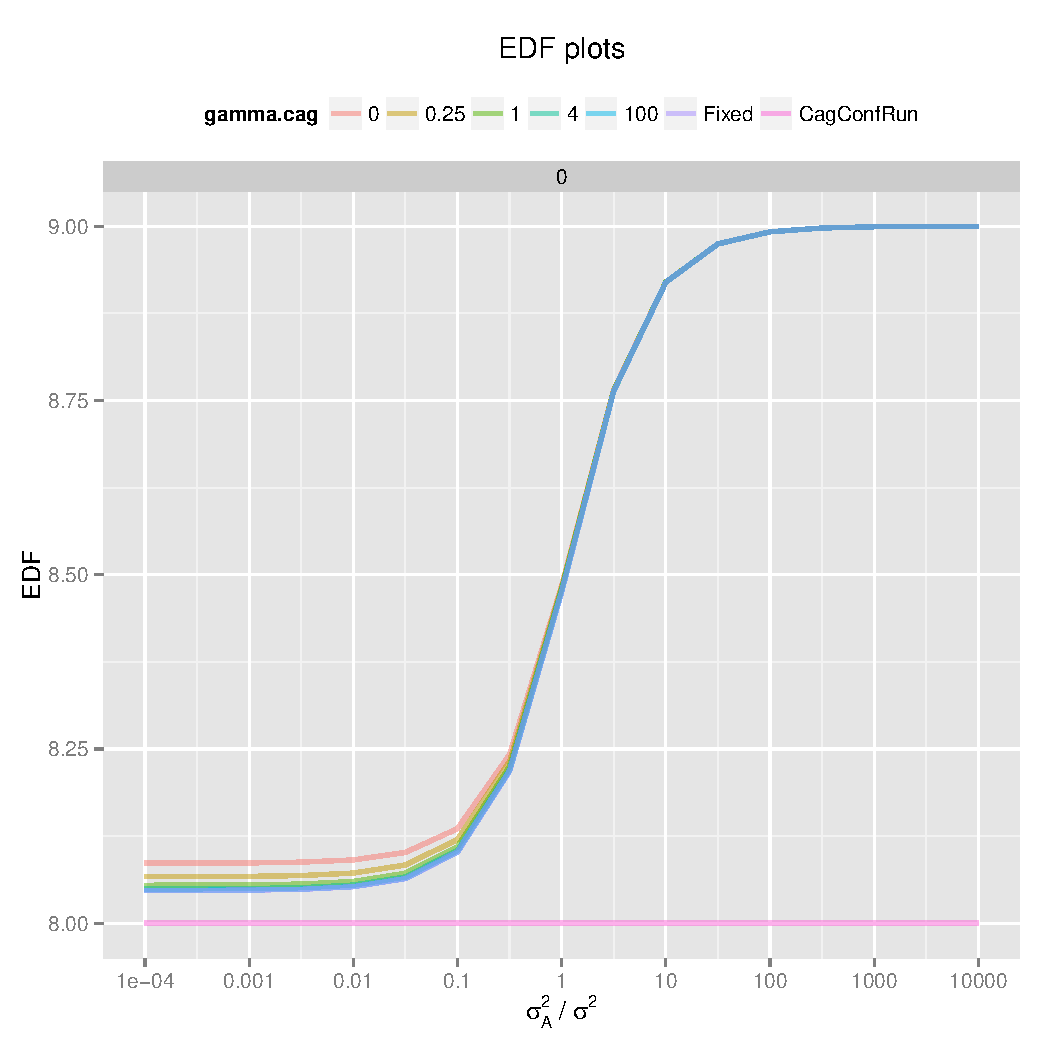
\includegraphics[width=.6 \textwidth]{Graph/RBD442Tag4EDFRun0.pdf}
\caption{Plots of EDF where the between runs VC is zero for the RBD experiments with $v = 4, r_b = 4$ and $n_B = 4$ comparing between different between cages VC estimates with the initial design where cages is confounded more with tags and the initial design where cages is confounded more with runs.}
\label{fig:RBD442Tag4EDFRun0}
\end{figure}

Comparing between the initial designs with 4-plex experiment, the design where the cages is confounded more with runs has better EDF when between animals VC is low and between runs VC is high, because the EDF is always at 8. If the VC of between animals is high and the between runs is low, the design where the cages is confounded more with tags should be considered, because the EDF can be as high as 9.

Figure~\ref{fig:RBD442Tag4vsTag8}, includes the EDF from the 8-plex experiments, gives an overall comparison in the EDF between the four designs. The two straight lines which are fixed at EDF of 8 and 7, are from the designs where cage is confounded more with runs in 4-plex and 8-plex experiments, respectively. Hence, there is no animal information can be recovered from the Between Runs stratum. As for the designs where the cage is confounded more with tags, the EDF can as high as 9, because the animal information can be recovered from the Between Run stratum. Between these four designs, the design with  where the cage is confounded more with tags and using 8-plex experiment is better, because the EDF are at least 8 under different VC and can be as high as 9 as the between animals VC increases.    

\begin{figure}[ht]
\centering
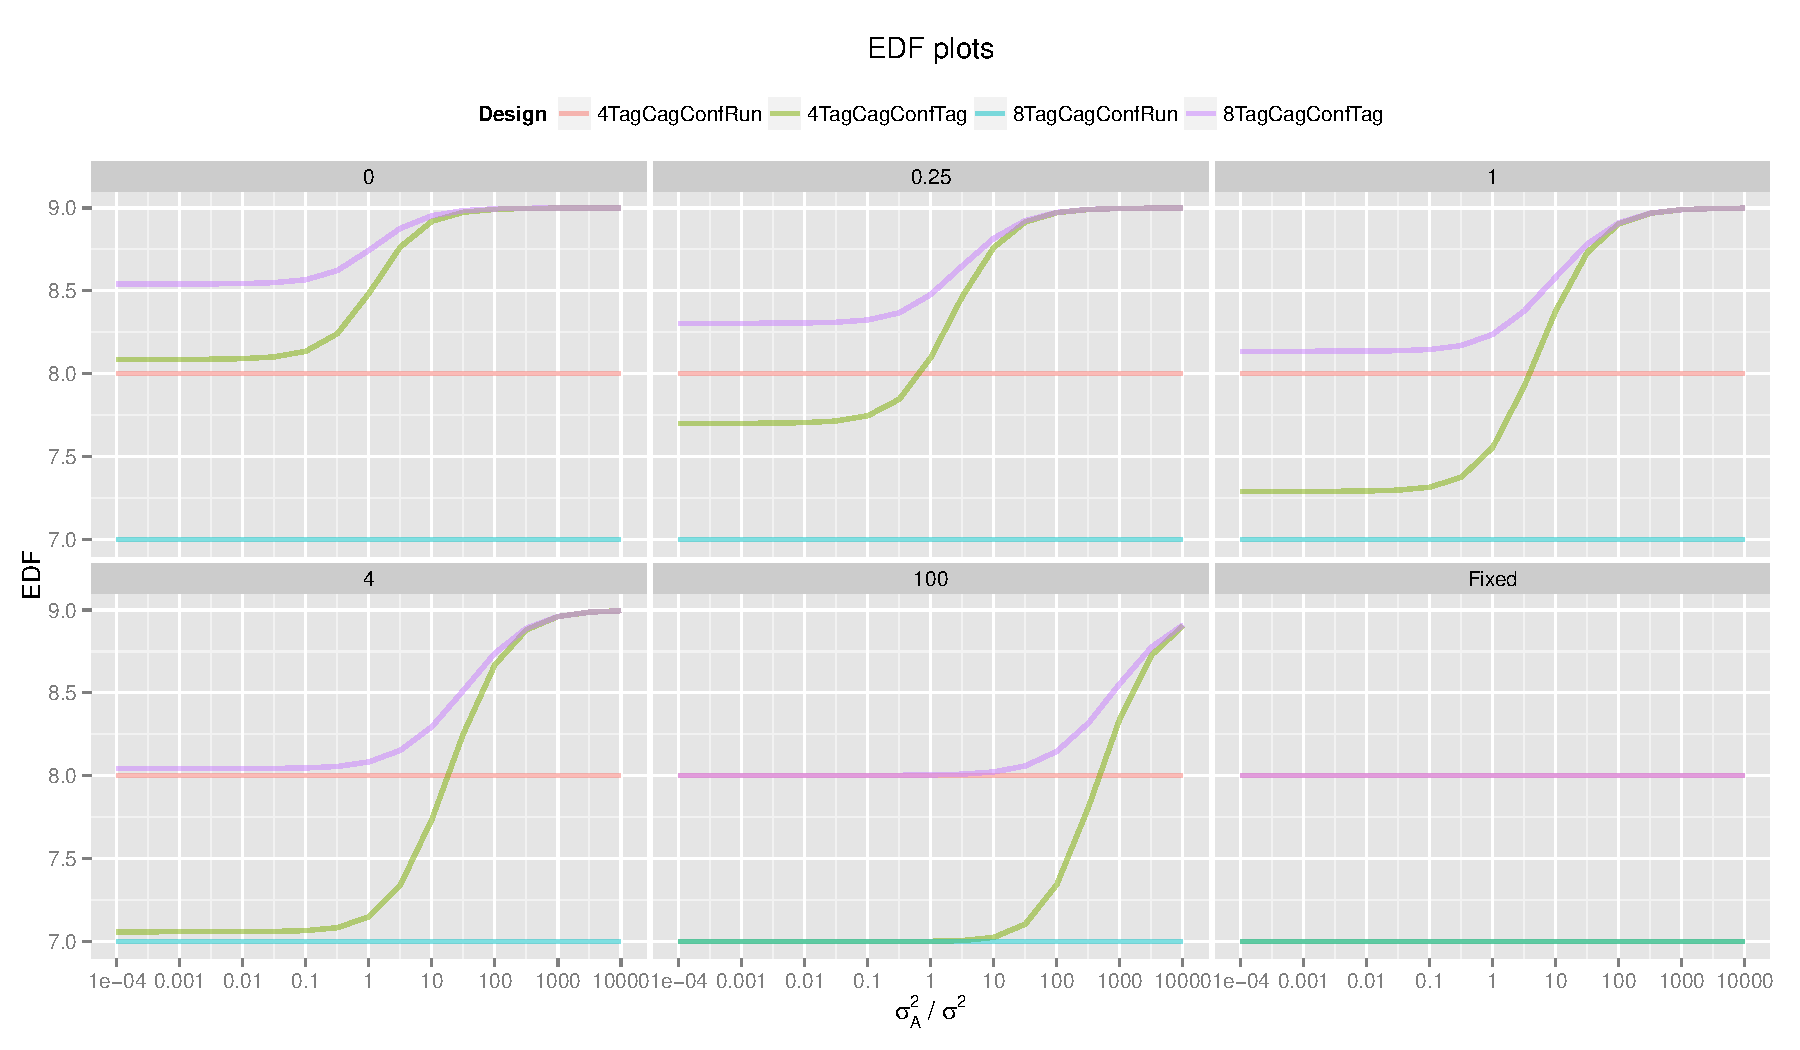
\includegraphics[width=1 \textwidth]{Graph/RBD442Tag4vsTag8.pdf}
\caption{Plots of EDF for the RBD experiments with $v = 4, r_b = 4$ and $n_B = 4$ comparing between the initial designs and between 4-plex and 8-plex experiments.}
\label{fig:RBD442Tag4vsTag8}
\end{figure}

This section shows the allocation of cages does affect the EDF. If the cage number is even, using the design where the cage is confounded more with tags is better, because it allows to have more DF associated with tag effects in the Between Cages stratum; thus, it maximised the overall DF associated Between Animals Within Cages strata in both Between and Within Runs strata. However, if the cage number is odd, the same guild line where the Phase 1 experiment is CRD can be followed instead.  

Recall from the previous section, the experiments with 4-plex system generally have 1 DF associated with Tag effect in the Between Animals Within Runs stratum, whereas the 8-plex system generally have 3 DF associated with tag effect in the Between Animals stratum. The 8-plex experiments can only be better than the 4-plex experiments if the experiment consists of 4 or 8 cages. This is because the cages can confounded all 3 DF of the tags effects and maximised the overall DF associated in the Between Animals Within Cages stratum as shown from the example given. As for the other examples of even cages, the 4-plex system should be considered. 

%I found that the VC of between cages does not affect the EDF. This is because the animals are nested from cages; thus, when the EMS consists of VC of between cages the given EMS should also consists of VCs of between animals.
%More specifically, when using experiment consist of even cages, but apart from 4 or 8 cages, 4-plex system is better than 8-plex system. It is because there is only 1 DF associated with cages that can be confounded with the tag effects. If the 4-plex system is used, it is possible to confound that the cages with that1 DF associated the tag effects; hence, the animals is then orthogonal to tags. If the 8-plex system is used, there is still at least 2 DF associated with the tag effects in the Between Animals Within Cages Within Runs stratum. e.g. $v = 2, r_b = 6, n_B  = 2, n_\gamma = 4$, EDF is between 7 and 9. $n_\gamma = 8$ EDF is between 6 and 7. 

\section{Compare the EDF where Phase 1 experiment is BIBD}
For the case where the Phase 1 experiment is BIBD, it follows the same guild line of the previous sections. Despite the Between Cages stratum have treatment information, the cage can still be allocated to confound more with either tag or run. 

As for the experiments comparing between 4 and 8 treatments, the 8-plex experiment is better that 4-plex experiment, because these two examples uses 4 and 8 cages, respectively.  

As for the experiments comparing between 5 and 7 treatments, since these two examples does not uses even number of cages; the guild line of CRD is used which means the 4-plex experiment is better than the 8-plex experiment. 

\section{Summary and Conclusion}
\label{sec:conclusion}
The chapter presents the LC and REML methods in estimating the VC. With the given VC estimates, the method in deriving the EDF is presented, this EDF is important because it is associated with the residual MS in the stratum where the tests for the treatment effects are conducted. 

The EDF are then compared between different optimal designs found where the Phase 1 experiment is arranged with CRD, RBD and BIBD. When the Phase 1 experiment is arranged with CRD, the EDF is better using 4-plex system compared to 8-plex system, because the 4-plex system contribute lesser DF associated with the tag effects which can be within the Between Animals Within Runs stratum. The 8-plex system is only better when comparing between 8 tags, because the treatment does not confound with animals in the Between Runs stratum. 

When the Phase 1 experiment is arranged with RBD or BIBD, the 4-plex system are still tend to have higher EDF. The 8-plex is again better when comparing between 8 treatment for the same reason as described in the example with CRD. The Phase 1 experiment also introduce an additional component of cages. The RBD example in Section~\ref{sec:expRBD} shows that it is the best to allocate the cages that is confounded more with tags, because it minimised the confounding of the animals with tags. Furthermore, when the Phase 1 experiment consists of 4 or 8 cages, it is shown to be the best to use 8-plex system, as the cages completely confounded 3 DF associated with tag effect which were in the Between Animals stratum as shown in the example presented.   

The chapter only presented the recovery of the random information from the Between Runs stratum. It is also possible to recover the treatment information. The optimal designs found from all cases have at least $80\%$ of the treatment average efficiency factor for conducting the test for the treatment effects. Hence, recovering the treatment information from the Between Runs stratum is not be necessary. 

%The R function getVcEDF() for estimating the VC and the EDF has developed.

\bibliographystyle{plainnat}
\bibliography{Reference/ref}

\end{document}
